\lhead{Capítulo \ref{ch_3}}
%\rhead{\newtitle}
\rhead{}
\cfoot{\thepage}
\renewcommand{\headrulewidth}{1pt}
\renewcommand{\footrulewidth}{1pt}
\chapter{Adaptación al Sitio en NOA}\label{ch_3}


En este capítulo se presentan los resultados obtenidos a partir de las distintas evaluaciones realizadas a la AS. 

\section{Medidas en tierra}


Los sitios analizados en esta tesis se resumen en la Tabla \ref{tab:sites}, donde se incluyen sus códigos de identificación, coordenadas geográficas, altitud sobre el nivel del mar, periodos de medición, clasificación climática según Köppen–Geiger \cite{peel2007} y el tipo de piranómetro utilizado. Estas estaciones  están ubicadas en el noroeste de Argentina como puede verse en la Figura \ref{fig:sites} y abarcan diversas condiciones climáticas y geográficas, que van desde tierras bajas subtropicales hasta altiplanos andinos de gran altitud.

\begin{figure}
   \centering
   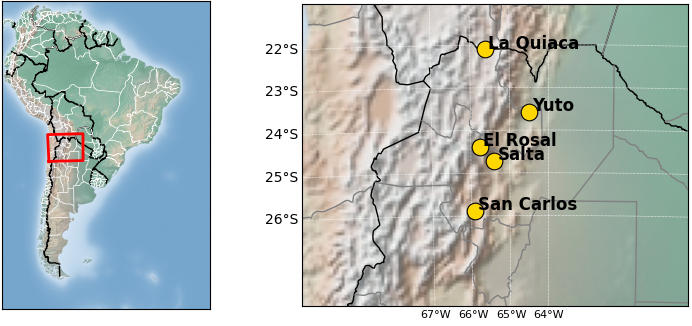
\includegraphics[width=1\linewidth]{figuras/sites.png}
    \caption{Ubicación de la estaciones de medida}
    \label{fig:sites}
\end{figure}


La estación Sa se encuentra en el campus experimental del INENCO, en la Universidad Nacional de Salta. Está situada en un entorno urbano preandino dentro del Valle de Lerma, una zona donde es común la formación de nubes debido a la cercanía de la cordillera. Su clima es subtropical de montaña, con inviernos secos y veranos frescos (Cwb). Las mediciones se realizaron entre 2009 y 2020 utilizando un piranómetro Eppley PSP.\\

La estación Lq, localizada en La Quiaca, presenta un clima estepario frío semiárido (BSk) típico de regiones andinas, y destaca por registrar uno de los mayores niveles de horas de sol anuales en Argentina. Contó con un piranómetro Kipp \& Zonen CMP11 y recopiló datos entre 2018 y 2023.

La estación Yu, ubicada en una zona de clima subtropical húmedo (Cwa), registró datos entre 2017 y 2018 con un sensor CMP11. La estación Sca, también con clima Cwb, operó entre 2012 y 2013 con un piranómetro CMP3. Finalmente, la estación Ero, situada en una región de gran altitud con clima BSk, recopiló datos entre 2016 y 2018, igualmente con un CMP3.

Todas las estaciones utilizan piranómetros que cumplen con los estándares de la norma ISO 9060:2018 Clase A o B para la medición de la irradiancia global horizontal (GHI). Los datos se registraron a intervalos de un minuto, y cada valor corresponde al promedio de seis muestras tomadas cada 10 segundos.




\begin{table}
    \centering
    \renewcommand{\arraystretch}{1.5} % Espaciado vertical en la tabla
    \begin{tabular}{|>{\centering\arraybackslash}p{2cm}|>{\centering\arraybackslash}p{2cm}|>{\centering\arraybackslash}p{2cm}|>{\centering\arraybackslash}p{2cm}|>{\centering\arraybackslash}p{2cm}|>{\centering\arraybackslash}p{2cm}|>{\centering\arraybackslash}p{2cm}|}
        \hline
        \textbf{ID} & \textbf{Provincia} & \textbf{Localidad} & \textbf{Latitud} & \textbf{Longitud}& \textbf{Altitud (m.s.n.m}) & \textbf{Clima}\\ 
        \hline

        \textbf{Yu} & Jujuy & Yuto & -23.58 & -64.5 & 401 & \textbf{Cwa}\\ 
        \textbf{Sa} & Salta & Salta & -24.72 & -65.4 & 1233 & \textbf{Cwb}\\ 
        \textbf{Sca} & Salta & San Carlos & -25.8951 & -65.925 & 1624 & \textbf{Cwb}\\
        \textbf{Er} & Salta & El Rosal & -24.39278 & -65.76806 & 3355& \textbf{Bsk}\\
        \textbf{Lq} & Jujuy & La Quiaca & -24.39278 & -65.76806 & 3355& \textbf{Bsk}\\
        \hline
        
        
    \end{tabular}
    \caption{Estaciones de medidas utilizadas en este trabajo}
    \label{tab:sites}
\end{table}




\subsection{Control de Calidad en las Medidas}

Las medidas fueron sometidas a un control de calidad (QC) siguiendo un procedimiento simplificado basado en \cite{Nollas2023}, con una etapa preliminar de filtrado por inspección visual según las recomendaciones de \cite{abal2020}. Dado que este estudio se basa únicamente en mediciones de irradiancia global horizontal (GHI) y no incluye componentes difusas, se aplicó una versión reducida del procedimiento original. 

La Tabla \ref{tab:qc} resume los filtros utilizados, donde $E$ es la constante solar, $S$ el factor de corrección de la distancia Tierra–Sol, $\theta_z$ el ángulo cenital solar y $kt$ el índice de claridad, definido como la razón entre la GHI y la irradiancia teórica en el tope de la atmósfera sobre un plano horizontal.\\

\begin{table}[h!]
\caption{Filtros de control de calidad aplicados a las mediciones.}
\label{tab:qc}
\centering
\resizebox{\linewidth}{!} {
\def\arraystretch{1.5}
\begin{tabular}{cc}
\hline
\textbf{Filtro} & \textbf{Descripción}\\ 
\hline
F1 & $GHI < 1.5~E~S~(\cos(\theta_z))^{1.2} + 100 \, \text{W/m}^2$  \\
F2 & $GHI > (6.5331 - 0.065502~\theta_z + 1.8312\text{E-4}~\theta_z^2)/(1 + 0.01113~\theta_z)$ \\
F3 & $kt < 1.4$ \& $ (90-\theta_z) < 10^\circ$  \\
\hline
\end{tabular}}
\end{table}

Los filtros aplicados pueden describirse de la siguiente manera:

\begin{itemize}
    \item \textbf{F1}: Rechaza valores que superan un límite físicamente razonable en función de la posición solar.
    \item \textbf{F2}: Descarta mediciones utilizando un umbral empírico dependiente del ángulo cenital.
    \item \textbf{F3}: Elimina valores del índice de claridad superiores a 1.4 cuando el Sol se encuentra a menos de $10^\circ$ sobre el horizonte.
\end{itemize}

El porcentaje de datos diurnos retenidos varió entre estaciones. En particular, el 73\% de los registros de Yu cumplieron los criterios establecidos, frente al 82\% en Sa, 72\% en Sca, aproximadamente 84\% en Ero y 69\% en Lq.





\subsection{Métricas de desempeño}

Los indicadores de desempeño más comunes en el campo de la evaluación del recurso solar han sido abordados por ~\cite{ZHANG}; estos incluyen el Error Medio de Sesgo (MBE), el Error Medio Absoluto (MAE) y el Error Cuadrático Medio (RMSE). Las tres métricas se definen de la siguiente manera:

\begin{equation}
\text{MBE} = \frac{\sum_{i=1}^{n} ( {y_i} - {x_i} ) }{n},
\end{equation}

\begin{equation}
\text{MAE} = \frac{\sum_{i=1}^{n} |{y_i} - {x_i} | }{n},
\end{equation}

\begin{equation}
\text{RMSE} = \sqrt{\frac{1}{n} \sum_{i=1}^{n} \Big({y_i - x_i}\Big)^2},
\label{ec:rrmsd}
\end{equation}

\noindent
donde $x$ y $y$ son los valores medidos y estimados, respectivamente, y $n$ es el tamaño de la muestra. El MBE mide el sesgo sistemático que un modelo puede introducir en una evaluación a largo plazo, mientras que el MAE y el RMSE miden la dispersión del error utilizando normas absolutas y cuadráticas, respectivamente. Debido a su mayor sensibilidad a los valores atípicos, el RMSE se utiliza frecuentemente en esta área. Ambas métricas de dispersión se reportan aquí por completitud. Los tres indicadores se presentan en términos relativos como un porcentaje del promedio de los valores medidos, denominados aquí como MBE (\%), MAE (\%) y RMSE (\%).




\section{Desempeño de los modelos de GHI en el NOA}
Previo a la presentación del desempeño de los distintos procesos de adaptación al sitio se evaluaron los modelos de estimación de GHI disponibles en la región. Siendo este uno de los aportes que se pretende en este trabajo. A continuación se muestran las métricas de desempeño de los modelos calculadas sobre el conjunto de datos de de cada sitio.



% Antes de la tabla, si quieres aumentar la altura de filas
\renewcommand{\arraystretch}{1.5}



\begin{table*}%[]
  \centering
  \caption{Métricas de desempeño (MBE, MAE, RMSE) para cada modelo y conjunto de datos satelitales en los cinco sitios. 
           Los valores están normalizados y expresados como porcentajes relativos al promedio de GHI en cada sitio: 
           396.8~W/m$^{2}$ (Yu), 397~W/m$^{2}$ (Sa), 557.1~W/m$^{2}$ (Sca), 690.6~W/m$^{2}$ (Ero) y 673.7~W/m$^{2}$ (Lq).}
  \resizebox{\linewidth}{!}{%
    \begin{tabular}{|l|ccc|ccc|ccc|ccc|ccc|}
      \hline
      & \multicolumn{3}{c|}{YU} & \multicolumn{3}{c|}{SA} & \multicolumn{3}{c|}{SCA} & \multicolumn{3}{c|}{ERO} & \multicolumn{3}{c|}{LQ} \\
      \cline{2-16}
      Modelo  & MBE & MAE & RMSE & MBE & MAE & RMSE & MBE & MAE & RMSE & MBE & MAE & RMSE & MBE & MAE & RMSE \\
      \hline
      \multicolumn{16}{|c|}{\textit{Resolución Temporal: 15 minutos}} \\
      \hline
      CAMS    & 0.5  & 18.4 & 28.4 & 3.5  & 23.9 & 33.2 & 2.7  & 23   & 30.4 & -23.7& 27.8 & 41.2 &-7.3 & 16.2 & 25.3 \\
      LSA-SAF & 10.7 & 19   & 28.8 & 17.3 & 26.9 & 38.8 & 11.5 & 22.2 & 30.6 & -8.1 & 16.5 & 26.8 & 3.7 & 12.3 & 22.3\\
      \hline
      \multicolumn{16}{|c|}{\textit{Resolución Temporal: horaria}} \\
      \hline
      CAMS    &  0.5 & 16   & 24.1 & 3.6  & 20.5 & 28.8 & 2.9  & 21   & 27.3 & -23.7& 26.8 & 39.5 & -6.1& 14.6 & 22\\
      LSA-SAF & 10.7 & 16.9 & 24.9 & 17.3 & 24.8 & 35   & 11.6 & 20.5 & 27.1 & -8.1 & 15   & 24.3 & 4.6 & 10.9 & 18.7\\
      ERA-5   & 0.4  & 22.7 & 34.6 & 8.5  & 26.8 & 37.5 & 7.4  & 21.2 & 28.9 & -13.7& 19.1 & 25.3 & -1.7& 12   & 19.3\\
      MERRA-2 & 26.9 & 35   & 51.9 & 42.1 & 47   & 63.6 & 12.7 & 21.9 & 29.3 & -3.1 & 13.1 & 20.5 & 1.0 & 13.4 & 21.1\\
      \hline
    \end{tabular}%
  }
\end{table*}
    


\subsection{Análisis de las estimaciones 15-minutales}

La Figura \ref{fig:general-15} muestra la evaluación comparativa de los modelos CAMS y LSA-SAF en los sitios de estudio. En el caso del MBE, se observa que LSA-SAF presenta sesgos positivos en la mayoría de los sitios, indicando una tendencia a la sobreestimación sistemática de las variables simuladas, mientras que CAMS exhibe valores más cercanos a cero o incluso negativos, lo que refleja un comportamiento más balanceado, aunque con subestimaciones marcadas en sitios como Er y Lq.


\begin{figure}
    \centering
    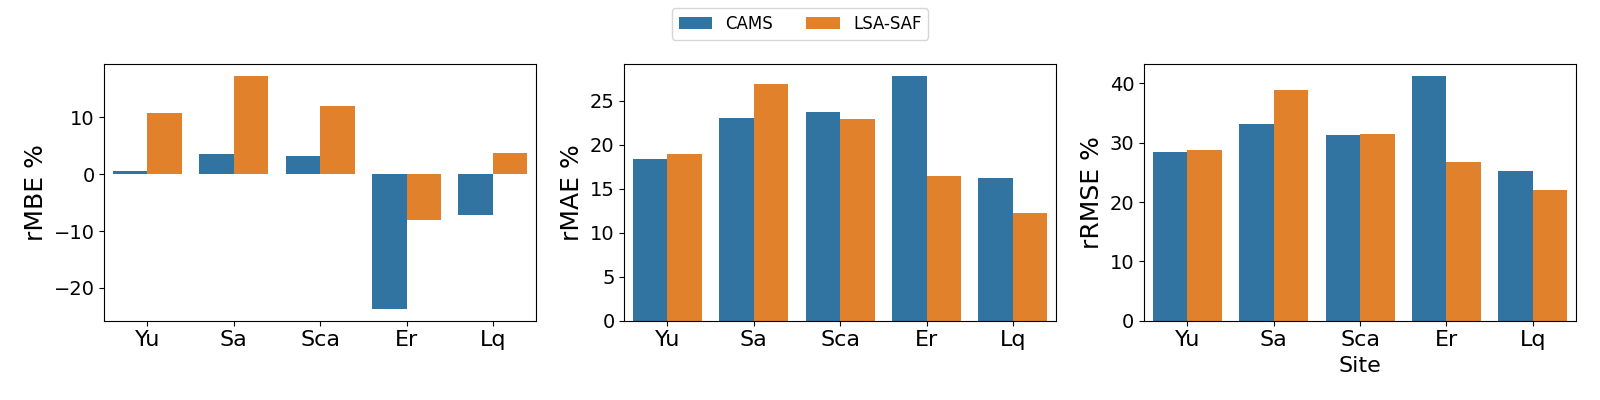
\includegraphics[width=\linewidth]{figuras/errors_15.png}
    \caption{Comparación del desempeño de los modelos CAMS y LSA-SAF en los cinco sitios de estudio (Yu, Sa, Sca, Er y Lq) mediante las tres métricas estadísticas: MBE, MAE y RMSE expresadas en términos porcentuales relativos a escala 15-minutal.}
    \label{fig:general-15}
\end{figure}

En relación al MAE, ambos modelos presentan magnitudes relativamente similares, aunque LSA-SAF tiende a mostrar errores absolutos ligeramente mayores en sitios como Yu y Sa, mientras que CAMS presenta valores más altos en Sca y Er. Esto sugiere que ninguno de los dos modelos logra una reducción clara y consistente del error en todos los sitios.\\

Por último, en la métrica RMSE, que penaliza los errores grandes, se mantiene un patrón semejante: LSA-SAF suele exhibir errores algo superiores a los de CAMS en Yu y Sa, mientras que en Er y Lq la diferencia favorece al modelo satelital. En general, los resultados muestran que el desempeño relativo de los modelos depende fuertemente del sitio, sin que exista un claro ganador en todos los casos.\\


\begin{figure} 
\centering 
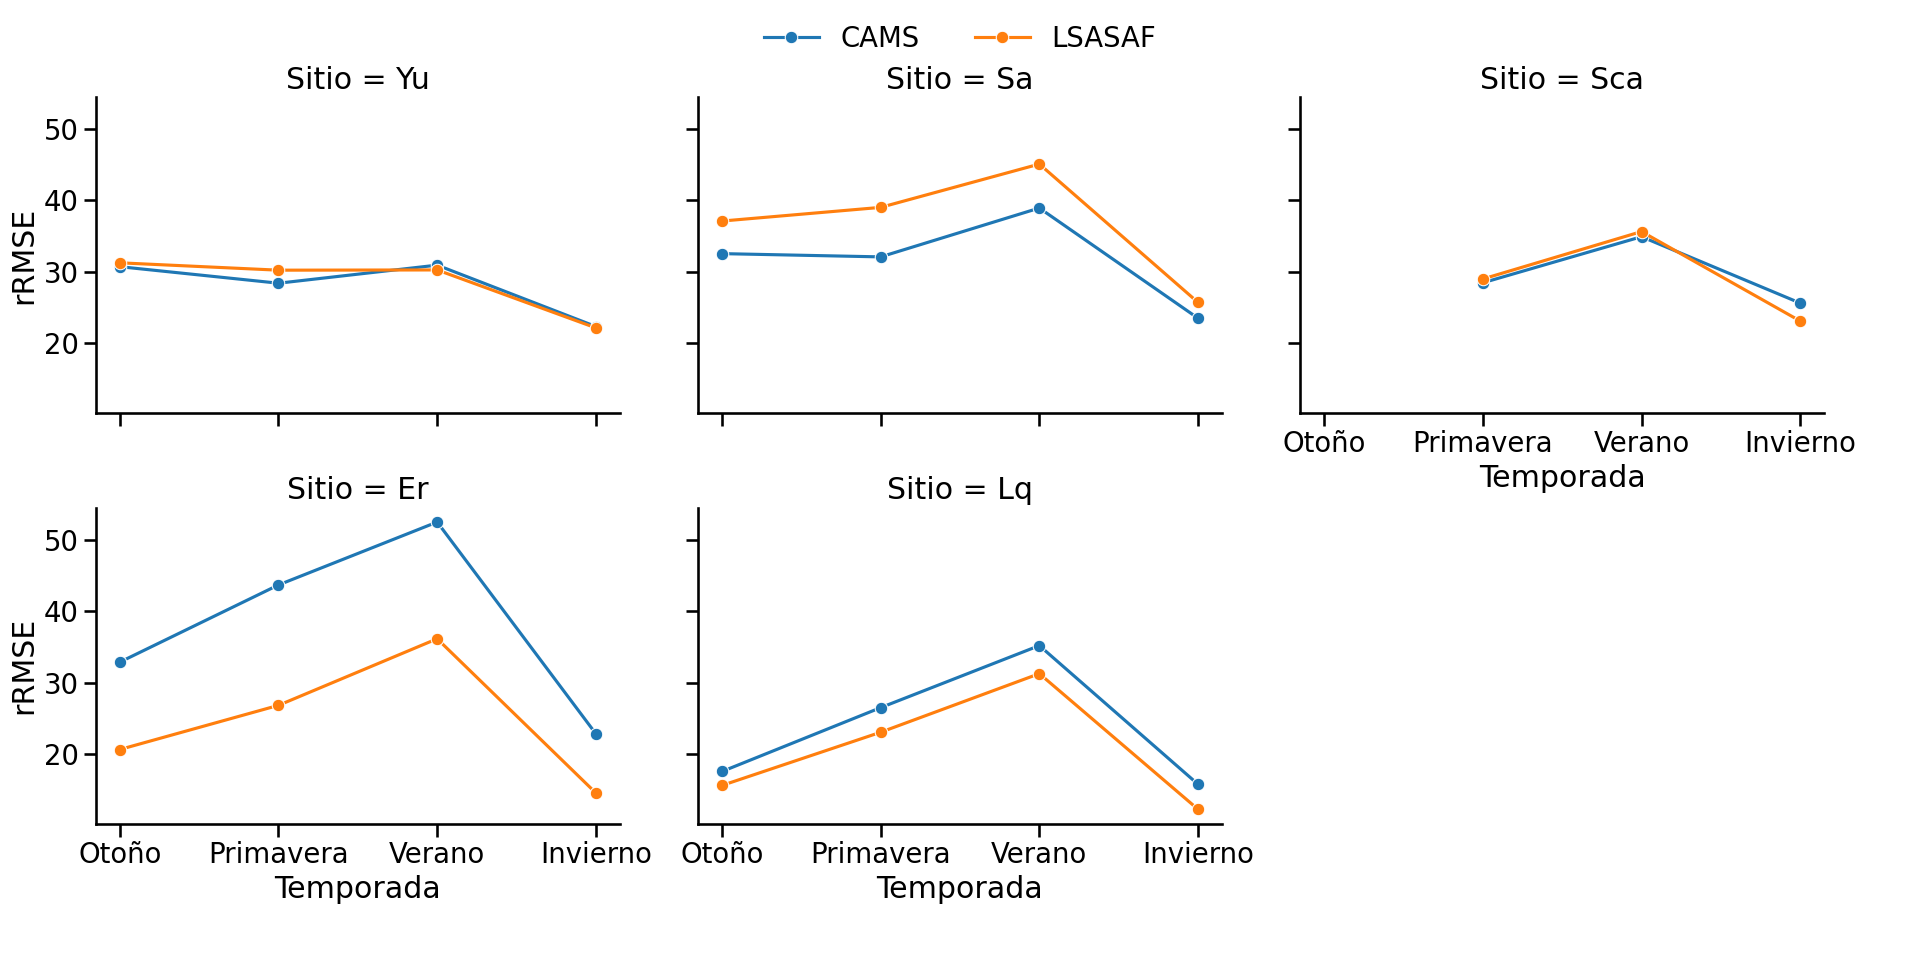
\includegraphics[width=\linewidth]{figuras/season_15_tesis.png}
 \caption{Figura \ref{fig:season-15}. Variación estacional del rRMSE (\%) para los productos CAMS y LSA-SAF con resolución de 15 minutos en todos los sitios de estudio. Se evidencia un aumento del error durante el verano en la mayoría de los sitios, mientras que en Yuto el rRMSE se mantiene estable, sugiriendo que la presencia de nubosidad estacional afecta de manera diferenciada la precisión de las estimaciones de radiación solar.} 
\label{fig:season-15} 
\end{figure}


La Figura \ref{fig:season-15} muestra la variación estacional del rRMSE (\%) para los productos CAMS y LSA-SAF con resolución de 15 minutos en todos los sitios de estudio. Se observa una clara tendencia estacional en el comportamiento del error: en general, el rRMSE tiende a aumentar durante el verano, lo que indica que la precisión de las estimaciones disminuye en este período en la mayoría de los sitios. La excepción es Yuto, donde el error permanece relativamente estable a lo largo de las estaciones. Este patrón sugiere que durante el verano hay una mayor presencia de nubosidad, lo cual podría estar afectando la capacidad de los modelos satelitales para estimar correctamente la radiación solar, mientras que en otras estaciones la cobertura nubosa es menor, permitiendo estimaciones más precisas.



En relación al MAE, ambos modelos presentan magnitudes relativamente similares, aunque LSA-SAF tiende a mostrar errores absolutos ligeramente mayores en sitios como Yu y Sa, mientras que CAMS presenta valores más altos en Sca y Er. Esto sugiere que ninguno de los dos modelos logra una reducción clara y consistente del error en todos los sitios.\\

Por último, en la métrica RMSE, que penaliza los errores grandes, se mantiene un patrón semejante: LSA-SAF suele exhibir errores algo superiores a los de CAMS en Yu y Sa, mientras que en Er y Lq la diferencia favorece al modelo satelital. En general, los resultados muestran que el desempeño relativo de los modelos depende fuertemente del sitio, sin que exista un claro ganador en todos los casos.\\



\begin{figure}
    \centering
    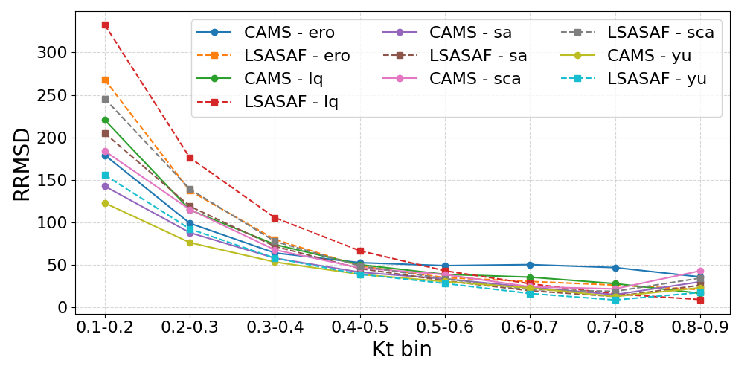
\includegraphics[width=\linewidth]{figuras/RMSE-kt-15.pdf}
    \caption{Variación del error cuadrático medio relativo (RRMSD) en función del indice de claridad (kt) para los cinco sitios analizados (YU, SA, SCA, ERO y LQ). Resultados para CAMS (líneas continuas) y LSASAF (líneas punteadas).}
    \label{fig:RMSE-kt-15}
\end{figure}



En el caso de RMSD vs Kt (Figura \ref{fig:RMSE-kt-15}), se observa una marcada disminución del error a medida que aumenta la claridad atmosférica. Para condiciones de cielo más nuboso (Kt < 0.3), los valores de RRMSD son elevados en todos los sitios, superando en algunos casos los 200 \%, especialmente en la estimación proveniente de LSASAF. Sin embargo, conforme Kt aumenta (>0.5), el error desciende rápidamente y tiende a estabilizarse por debajo del 50\%, alcanzando valores mínimos en condiciones de cielo despejado (Kt > 0.7). Esta tendencia se mantiene consistente en ambos productos (CAMS y LSASAF), aunque LSASAF presenta errores relativamente mayores en las condiciones más turbias.




\begin{figure}
    \centering
    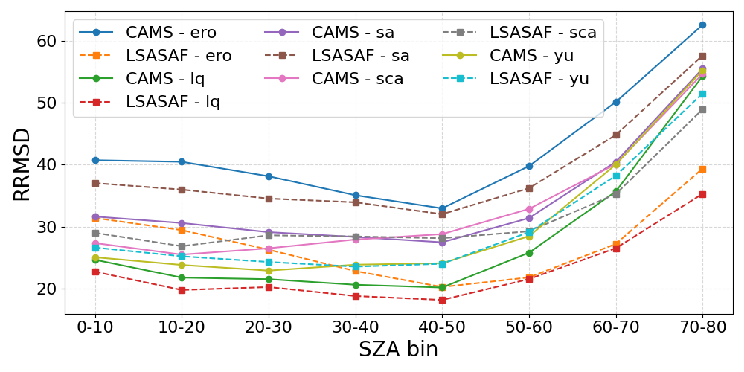
\includegraphics[width=0.8\textwidth]{figuras/RMSE-sza-15.pdf}
    \caption{Variación del error cuadrático medio relativo (RRMSD) en función del ángulo cenital solar (SZA) para los cinco sitios analizados (YU, SA, SCA, ERO y LQ). Resultados para CAMS (líneas continuas) y LSASAF (líneas punteadas).}
    \label{fig:RMSE-SZA-15}
\end{figure}



Por otro lado, la relación RRMSD vs SZA (Figura \ref{fig:RMSE-SZA-15}) evidencia un comportamiento en forma de “U” invertida: los menores errores se concentran en ángulos intermedios (30°–50°), mientras que hacia ángulos bajos (<20°) y altos (>70°) el error aumenta de manera significativa. Esta tendencia se observa en los cinco sitios, con un incremento más pronunciado en ERO y SA en las condiciones de SZA más extremas. En general, CAMS muestra un mejor desempeño que LSASAF en la mayoría de los intervalos, aunque las diferencias se reducen en los ángulos medios.

En conjunto, estos resultados indican que la precisión de ambos productos depende fuertemente de las condiciones atmosféricas (Kt) y de la geometría solar (SZA). En cielos despejados y ángulos intermedios, los errores se reducen notablemente, mientras que en condiciones nubosas y en situaciones de baja o alta elevación solar los modelos presentan las mayores limitaciones.


\subsection{Análisis de las estimaciones horarias}

La Figura \ref{fig:general-60} presenta la evaluación comparativa del desempeño de los modelos satelitales CAMS y LSA-SAF, junto con los reanálisis ERA5 y MERRA-2, a escala horaria. En términos generales, se observa que tanto los modelos satelitales como los de reanálisis muestran un comportamiento con aparente dependencia de las condiciones de nubosidad del sitio. En localidades con predominio de cielo despejado, ambos tipos de modelos tienden a mostrar un desempeño similar, con la excepción del modelo CAMS en Ero, cuyo comportamiento particular se discute de manera separada. Por el contrario, en sitios con condiciones de nubosidad más variables, los modelos de reanálisis tienden a presentar un desempeño inferior en comparación con los modelos satelitales. Estas métricas son coincidentes con los reportes ya documentados sobre el desempeño de estos modelos en la región \citep{Ledesma2025}.\\

\begin{figure}
    \centering
    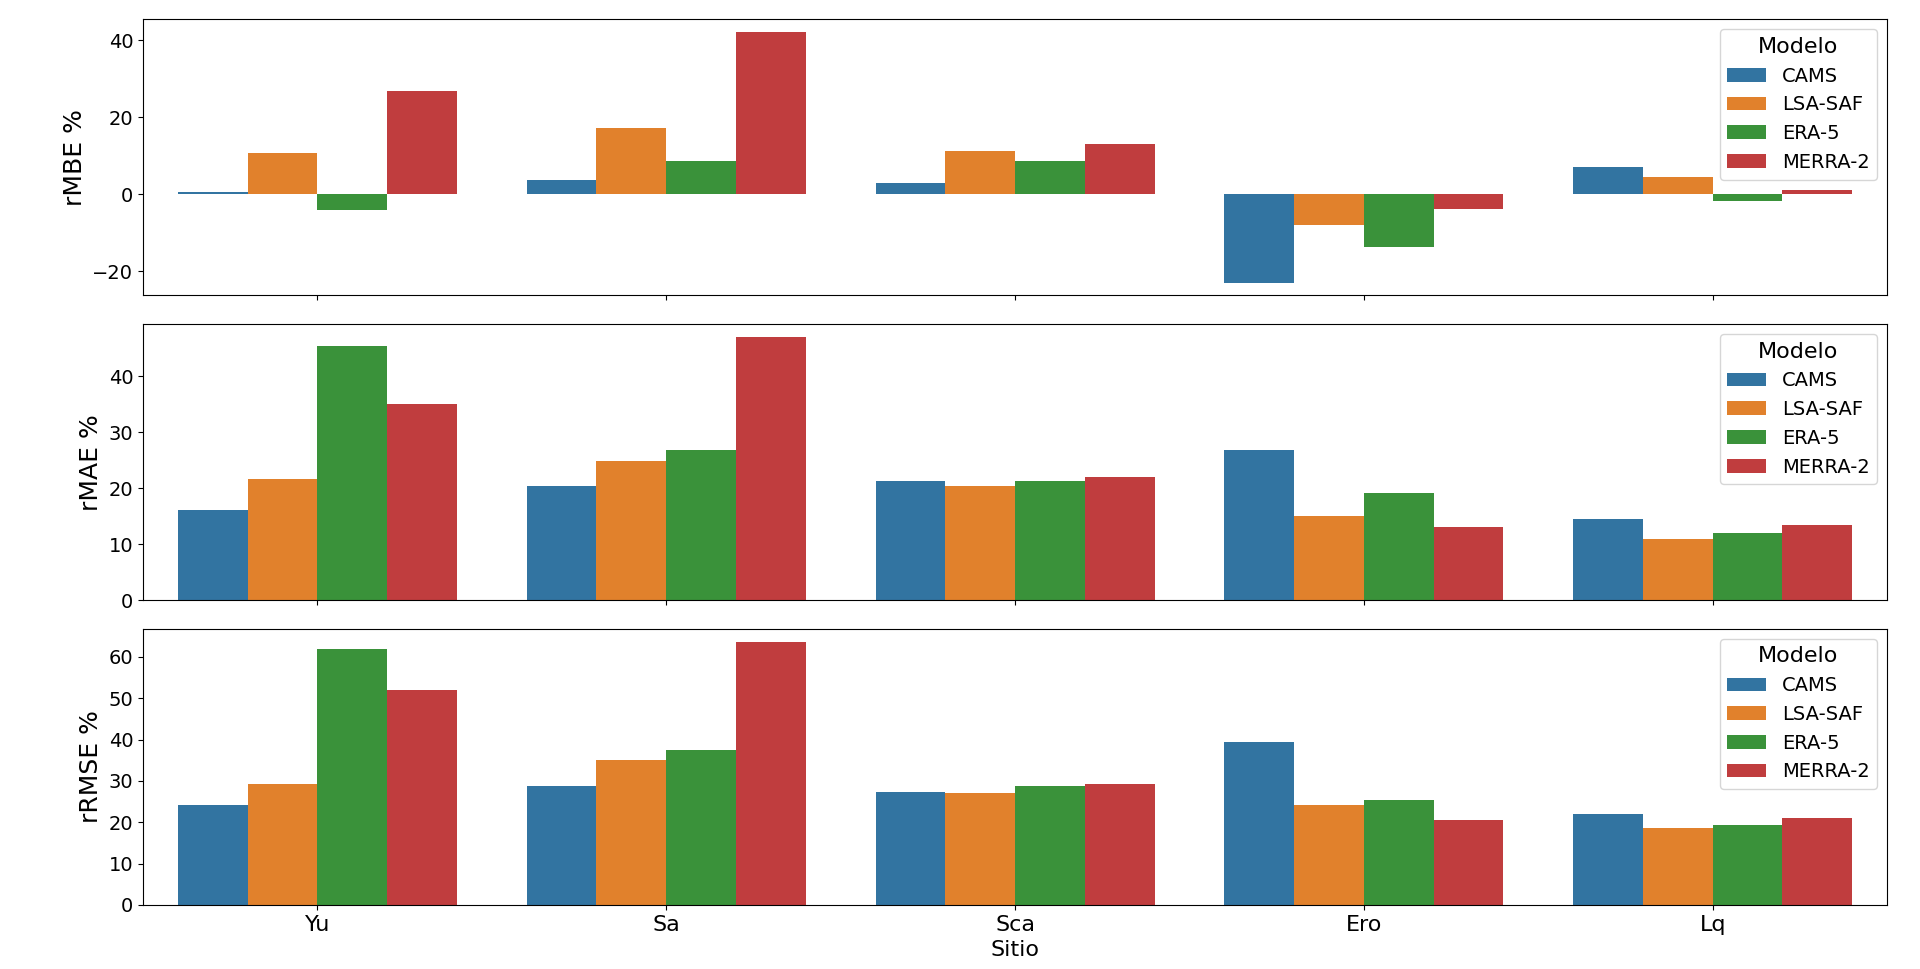
\includegraphics[width=\linewidth]{figuras/errors_60.png}
    \caption{Comparación del desempeño de los modelos satelitaltes CAMS y LSA-SAF y de re-análisis en los cinco sitios de estudio (Yu, Sa, Sca, Er y Lq) mediante las tres métricas estadísticas: MBE, MAE y RMSE expresadas en términos porcentuales relativos a escala horaria.}
    \label{fig:general-60}
\end{figure}


En Ero, el modelo de CAMS presenta un comportamiento atípico en su estimación. Como se observa en la Figura \ref{fig:ero}, el modelo tiende a sobreestimar la nubosidad. Este problema ya ha sido documentado por los propios desarrolladores y se ha reportado un comportamiento similar en un sitio desértico \cite{qu2017}. Según los autores, el modelo tiene dificultades para clasificar correctamente ciertos instantes despejados, que son identificados erróneamente como nubosos. Esto ocurre porque un píxel desértico puede aparecer frío en el canal térmico y brillante en el visible, lo que provoca falsos positivos de nubes en el algoritmo APOLLO/SEV.


\begin{figure}
    \centering
    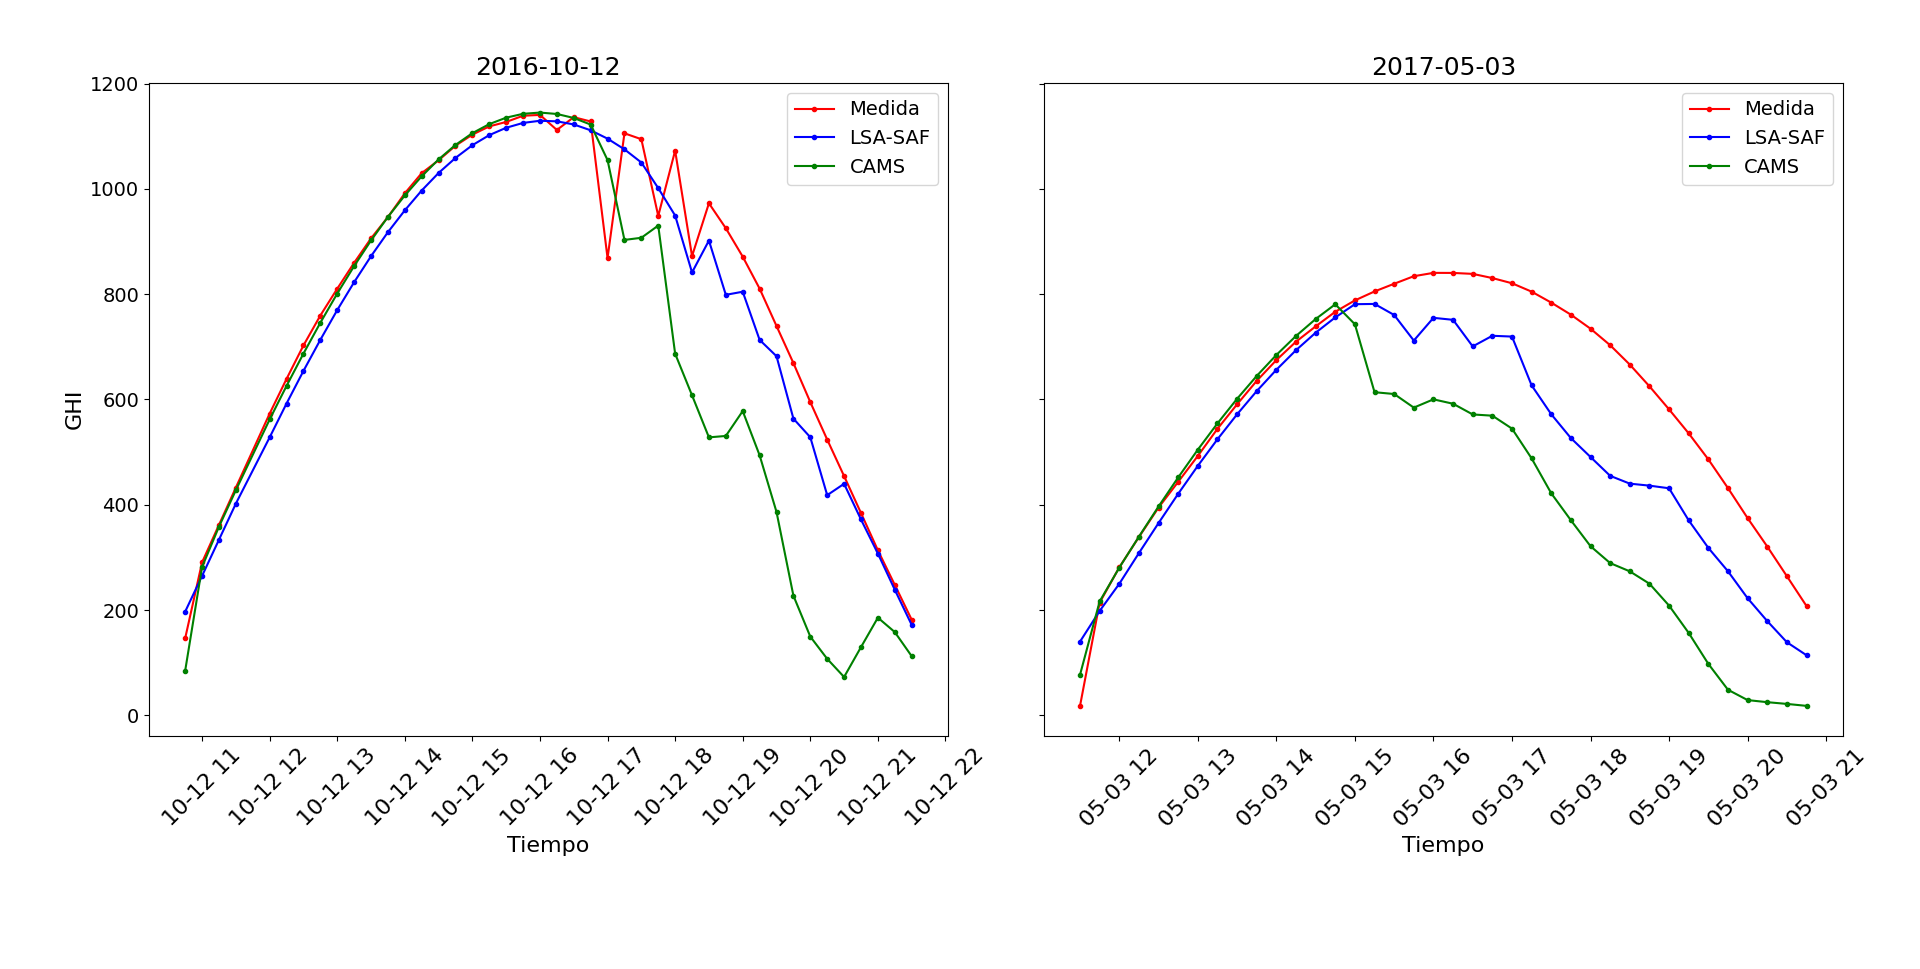
\includegraphics[width=\linewidth]{figuras/ero.png}
    \caption{Comparación de la serie de GHI medida frente a las estimaciones de los modelos LSA-SAF y CAMS para dos días en Ero.}
    \label{fig:ero}
\end{figure}





\subsection{División del conjunto de datos}
De acuerdo a lo indicado en la sección \ref{MLM} el conjunto de datos debe ser segmentado con fin de evaluar el rendimiento de los modelos de aprendizaje automático utilizados en la regresión del proceso de adaptación al sitio y controlar el sobre-entrenamiento de los modelos. En el contexto de AS en los trabajos \cite{POLO2016, POLO2020} se recomienda tomar al menos un año de medidas para la calibración de los modelos. Siguiendo estas ideas el conjunto de medidas fue dividido en subconjunto de entrenamiento, validación y prueba.  


\begin{table}[ht]
    \centering
    \renewcommand{\arraystretch}{1.5} % Espaciado vertical en la tabla
    \begin{tabular}{|>{\centering\arraybackslash}p{2cm}|>{\centering\arraybackslash}p{3cm}|>{\centering\arraybackslash}p{3cm}|>{\centering\arraybackslash}p{4cm}|}
        \hline
        \textbf{ID} & \textbf{Entrenamiento} & \textbf{Validación} & \textbf{Prueba}\\ 
        \hline

        \textbf{YU}  & 2017 & 2017 & 2018 \\ 
        \textbf{SA}  & 2009 & 2009 & 2010 - 2024 \\ 
        \textbf{SCA} & 2013 & 2013 & 2012-2014 \\
        \textbf{ERO} & 2013 & 2013 & 2014 - 2024  \\
        \textbf{LQ}  & 2019 & 2019 & 2018, 2021 - 2023  \\
    \hline
    \end{tabular}
    \caption{División del conjunto de datos en entrenamiento, validación y prueba }
    \label{tab:tvt}
\end{table}

    



\begin{table*}%[]
  \centering
  \label{tbl:metrics_test}
  \caption{Métricas de desempeño (MBE, MAE, RMSE) para cada modelo y conjunto de datos satelitales en los cinco sitios en el \textbf{conjunto de pruebas}. 
           Los valores están normalizados y expresados como porcentajes relativos al promedio de GHI en cada sitio: 
           396.8~W/m$^{2}$ (Yu), 397~W/m$^{2}$ (Sa), 557.1~W/m$^{2}$ (Sca), 690.6~W/m$^{2}$ (Ero) y 673.7~W/m$^{2}$ (Lq).}
  \resizebox{\linewidth}{!}{%
    \begin{tabular}{|l|ccc|ccc|ccc|ccc|ccc|}
      \hline
      & \multicolumn{3}{c|}{YU} & \multicolumn{3}{c|}{SA} & \multicolumn{3}{c|}{SCA} & \multicolumn{3}{c|}{ERO} & \multicolumn{3}{c|}{LQ} \\
      \cline{2-16}
      Modelo  & MBE & MAE & RMSE & MBE & MAE & RMSE & MBE & MAE & RMSE & MBE & MAE & RMSE & MBE & MAE & RMSE \\
      \hline
      \multicolumn{16}{|c|}{\textit{Resolución Temporal: 15 minutos}} \\
      \hline
      CAMS    & -0.2 & 17.4 & 27.2 & 3.9  & 23.4 & 33.7 & 2.6  & 21.8 & 29.8 & -23.6 & 27.6 & 40.9 & -6.9 & 16.5 & 25.8 \\
      LSA-SAF & 7.6  & 16.5 & 25.5 & 17.9 & 27.4 & 39.4 & 13.1 & 22.2 & 30.9 & -7.7  & 16.2 & 26.5 & 4.0  & 12.6 & 22.6 \\
      \hline
      \multicolumn{16}{|c|}{\textit{Resolución Temporal: horaria}} \\
      \hline
      CAMS    & 0.9  & 16.6 & 24.6 & 4.0 & 20.9 & 29.3 & 3.0 & 19.7 & 26.1 & -23.6 & 26.6 & 39.3 & -4.8 & 14.5 & 21.6 \\
      LSA-SAF & 12.6 & 18.5 & 26.6 & 17.9 & 25.3 & 35.7 & 13.3 & 20.3 & 27.1 & -7.7  & 14.8 & 24.0 & 4.8  & 10.9 & 18.2 \\
      ERA-5   & -1.0 & 23.1 & 35.2 & 9.4  & 27.1 & 37.7 & 1.9  & 20.2 & 29.7 & -14.0 & 19.3 & 25.6 & -0.8 & 11.3 & 18.4 \\
      MERRA-2 & 28.1 & 36.0 & 52.4 & 43.4 & 48.3 & 65.0 & 10.9 & 21.7 & 30.3 & -3.8  & 13.1 & 20.4 & 1.4  & 13.4 & 20.8 \\
      \hline
    \end{tabular}%
  }
\end{table*}

    



\section{Adaptación al sitio con una variable descriptiva}\label{sec:01}


En los trabajos citados en la Sección \ref{ch_3} sobre la evaluación del proceso de Adaptación al Sitio (SA), se ha prestado escasa atención a las razones subyacentes por las cuales ciertos modelos de aprendizaje automático (ML) superan a otros en este proceso. Dado que algunos modelos de ML poseen una naturaleza inherentemente más compleja que otros, podría suponerse que los modelos más complejos ofrecerían un rendimiento superior frente a aquellos de menor complejidad. En este contexto, el término complejidad hace referencia tanto a la complejidad computacional —es decir, la cantidad de operaciones necesarias para ejecutar el modelo— como a la complejidad conceptual, relacionada con el nivel de conocimiento requerido para comprender su funcionamiento.\\

En esta sección se presenta una implementación del proceso de SA basada en uno de los enfoques clásicos, que consiste en adaptar una serie temporal modelada (proveniente de datos satelitales o de reanálisis) utilizando como referencia una serie de mediciones in situ.\\

Dado que el modelo de Regresión Lineal Simple (RLS) puede considerarse el menos complejo entre los empleados en este estudio, la primera evaluación del proceso de SA en la región de interés se realiza utilizando este modelo. El objetivo es comparar el desempeño de la RLS con el de modelos de regresión más complejos, como el Perceptrón Multicapa (MLP) y XGBoost, utilizando las mismas métricas de evaluación.\\

Para los modelos MLP y XGBoost, la determinación de la configuración óptima de hiperparámetros fue fundamental para lograr un desempeño consistente en las particiones de validación cruzada. Esto se llevó a cabo mediante una búsqueda exhaustiva en rejilla (Grid Search) implementada con la función \textbf{GridSearchCV} de la biblioteca \textbf{Scikit-learn} en Python \cite{Pedregosa2012}. Los rangos específicos de hiperparámetros evaluados para MLP y XGBoost se presentan en la Tabla \ref{tab:gridsearch}. La selección de hiperparámetros óptimos constituye un paso crítico en el aprendizaje automático, ya que influye directamente en la complejidad del modelo, su capacidad de generalización y su rendimiento predictivo global \cite{Goodfellow2016}.\\



\begin{table}[ht]
\caption{Espacio cartesiano de hiperparámetros para las técnicas de aprendizaje supervisado.}
\label{tab:gridsearch}
\centering
\resizebox{\linewidth}{!} {
\def\arraystretch{1.5}
\begin{tabular}{lcccc}
\hline
\textbf{Hiperparámetro} & \textbf{Inferior} & \textbf{Superior} & \textbf{Paso} & \textbf{Función de transformación} \\
\hline
MLP\\
\hline
 Capas ocultas        & 1    & 3     & 1   & - \\
 Nodos ocultos        & 1    & 4     & 1   & $2^{x}$ \\
 Fracción de dropout  & 0    & 0.3   & 0.1 & - \\
 Tasa de aprendizaje  & -3   & -1    & 1   & $10^{x}$ \\
\hline
XGBoost\\
\hline
Booster               & gbtree & & & \\
 Estimadores          & 1    & 50    & 10  & - \\
 Profundidad máxima   & 2    & 5     & 1   & $2^{x}$ \\
 Tasa de aprendizaje  & -3   & -1    & 1   & $10^{x}$ \\
\hline
\end{tabular}}
\end{table}

En cuanto al preprocesamiento de los datos de entrada, la normalización o el escalado de características es una práctica común en aprendizaje automático para mejorar la convergencia y la estabilidad, particularmente en modelos sensibles a la magnitud de las variables de entrada. Sin embargo, en este estudio \textbf{no se aplicó normalización}, ya que no se consideró necesaria para los modelos y datos utilizados.  

En el caso del modelo \textbf{SLR}, el escalado de la variable independiente no es necesario porque el modelo es inherentemente invariante al escalado: multiplicar la entrada por un factor constante provoca un cambio inversamente proporcional en el coeficiente de la pendiente, dejando las predicciones sin alterar.  

De manera similar, \textbf{XGB}, cuando se implementa con árboles de decisión como aprendices base, \textbf{no requiere escalado de características}, ya que las divisiones en los nodos dependen del \textbf{orden relativo} de los valores y no de sus magnitudes absolutas \cite{Soria2022, Chen2016}.  

En el caso del modelo \textbf{MLP}, el escalado puede ser importante cuando las variables de entrada difieren significativamente en su rango o unidades. Sin embargo, en el presente estudio se utilizó \textbf{una sola variable de entrada} (GHI derivado de satélite), expresada en las \textbf{mismas unidades y rango} que la variable objetivo (GHI medido en superficie). Por lo tanto, no se consideró necesaria ninguna normalización adicional.

Los resultados obtenidos son expresados en la Tabla \ref{tab:metrics-as-1}.


\begin{table*}%[]
  \centering
  \label{tab:metrics-as-1}
  \caption{Métricas de desempeño (MBE, MAE, RMSE) para cada modelo adaptado en los cinco sitios en el \textbf{conjunto de pruebas}}
  \resizebox{\linewidth}{!}{%
    \begin{tabular}{|l|ccc|ccc|ccc|ccc|ccc|}
      \hline
      & \multicolumn{3}{c|}{YU} & \multicolumn{3}{c|}{SA} & \multicolumn{3}{c|}{SCA} & \multicolumn{3}{c|}{ERO} & \multicolumn{3}{c|}{LQ} \\
      \cline{2-16}
      Modelo  & MBE & MAE & RMSE & MBE & MAE & RMSE & MBE & MAE & RMSE & MBE & MAE & RMSE & MBE & MAE & RMSE \\
      \hline
      \multicolumn{16}{|c|}{\textit{Resolución Temporal: 15 minutos}} \\
      \hline
      CAMS SLR    & -0.9 & 17.1 & 26.4 &  3.8 & 21.3 & 31.5 & -1.5 & 18.4 & 26.0 &  2.5 & 24.8 & 31.5 &  2.1 & 15.9 & 23.5 \\
      CAMS MLP    & -4.4 & 17.7 & 26.2 &  4.8 & 21.4 & 31.6 &  7.7 & 17.8 & 27.7 &  0.5 & 24.1 & 31.2 &  9.1 & 19.4 & 25.6 \\
      CAMS XGB    & -1.3 & 17.1 & 26.0 &  3.8 & 21.4 & 31.4 & -1.8 & 18.9 & 26.2 &  2.5 & 23.9 & 30.9 &  2.2 & 15.9 & 23.5 \\
      \hline
      LSASAF SLR  & -5.5 & 18.4 & 25.0 &  4.4 & 23.9 & 34.6 &  1.0 & 18.0 & 26.7 &  2.7 & 17.1 & 25.4 &  2.2 & 12.9 & 22.3 \\
      LSASAF MLP  & -7.1 & 18.6 & 25.0 &  4.5 & 23.6 & 34.5 &  5.9 & 18.4 & 26.6 &  2.5 & 17.0 & 25.3 & -0.4 & 13.6 & 22.1 \\    
      LSASAF XGB  & -6.0 & 18.2 & 24.9 &  4.3 & 23.9 & 34.6 &  0.5 & 18.6 & 27.0 &  2.4 & 17.2 & 25.1 &  2.3 & 13.1 & 22.3 \\
      \hline
      \multicolumn{16}{|c|}{\textit{Resolución Temporal: horaria}} \\
      \hline
      CAMS SLR    &  0.4 & 16.2 & 23.8 &  3.5 & 18.5 & 27.0 & -1.7 & 15.9 & 22.0 &  2.1 & 23.4 & 29.6 &  2.6 & 13.8 & 19.4 \\
      LSASAF SLR  &  5.2 & 16.5 & 24.1 &  4.3 & 21.2 & 30.5 &  1.1 & 15.6 & 22.7 &  2.5 & 15.7 & 22.8 &  0.3 & 10.6 & 17.4 \\
      ERA-5 SLR   & -2.7 & 23.2 & 35.2 &  6.4 & 26.5 & 36.9 & -6.4 & 20.1 & 29.1 & -0.6 & 15.4 & 21.4 &  2.1 & 11.6 & 18.4 \\
      MERRA-2 SLR &  2.3 & 33.6 & 43.4 &  7.1 & 35.2 & 46.0 & -2.2 & 20.3 & 27.7 &  0.7 & 12.9 & 20.1 &  0.3 & 13.1 & 20.4 \\
      \hline
      CAMS MLP    & 0.3 & 16.3 & 23.6 &  4.3 & 18.6 & 27.2 & -4.0 & 16.6 & 22.4 &  3.8 & 23.5 & 29.5 & -0.5 & 13.0 & 19.2 \\
      LSASAF MLP  & 5.6 & 16.4 & 23.7 &  2.5 & 21.4 & 30.2 &  8.3 & 16.1 & 24.1 &  9.6 & 19.4 & 24.6 & -3.8 & 12.1 & 17.8 \\
      ERA-5 MLP   & 0.0 & 23.2 & 35.2 &  9.6 & 27.1 & 37.6 & -1.8 & 19.0 & 28.5 & -7.5 & 16.7 & 23.1 &  0.1 & 11.3 & 18.3 \\
      MERRA-2 MLP & 1.4 & 34.0 & 43.4 &  0.8 & 36.3 & 45.4 & -0.3 & 19.5 & 27.5 & 11.7 & 17.5 & 23.4 & -2.8 & 13.4 & 20.6 \\
      \hline
      CAMS XGB    & 0.8  & 16.5 & 23.7 &  3.4 & 18.9 & 27.1 & -2.4 & 16.6 & 22.4 &  2.1 & 22.8 & 29.2 &  2.7 & 13.9 & 19.6 \\
      LSASAF XGB  & 4.9  & 16.5 & 23.7 &  4.1 & 21.4 & 30.6 &  0.0 & 16.9 & 23.4 &  2.2 & 15.9 & 22.6 &  0.2 & 10.9 & 17.4 \\
      ERA-5 XGB   & -1.5 & 24.3 & 35.2 &  6.3 & 27.3 & 37.4 & -7.3 & 20.7 & 29.3 & -0.5 & 15.2 & 21.2 &  2.0 & 11.8 & 18.6 \\
      MERRA-2 XGB & 2.8  & 34.8 & 44.1 & 6.9 & 35.6 & 46.1 & -2.8 & 20.8 & 28.2 &  0.8 & 13.3 & 20.3 &  0.2 & 13.5 & 20.6 \\
      \hline
    \end{tabular}%
  }
\end{table*}

La evaluación comparativa de los modelos SLR,MLP y XGB, utilizando como variables de entrada los productos satelitales \textit{CAMS} y \textit{LSA-SAF}, se realizó en cinco sitios con características climáticas y geográficas diversas. El desempeño se expresó en términos de error medio de sesgo (MBE), error absoluto medio (MAE) y raíz del error cuadrático medio (RMSE), todos normalizados respecto al promedio de la irradiancia global horizontal (GHI) en cada estación (Tablas~\ref{tab:metrics-as-1} y \ref{tbl:metrics_test}).  

En términos generales, los errores normalizados se mantuvieron dentro de un rango moderado en todas las combinaciones de modelos y conjuntos de datos, sin observarse diferencias sustanciales entre los enfoques lineales y los no lineales. El modelo RLS mostró un desempeño competitivo en ambos conjuntos de datos, con métricas de error cercanas a las obtenidas por los modelos más complejos.  

En el caso de \textbf{CAMS}, aunque el MLP logró reducir ligeramente el RMSE en algunos sitios, esto se produjo a costa de sesgos más pronunciados en el MBE, lo cual evidencia una compensación entre reducción de varianza e incremento del error sistemático. El modelo XGB, por su parte, presentó un comportamiento muy similar al de RLS, con diferencias marginales.  

Por otro lado, al emplear \textbf{LSA-SAF} se observó una ligera mejora respecto a CAMS, particularmente en estaciones de mayor altitud (ERO y LQ), donde tanto XGB como MLP alcanzaron menores valores de MAE y RMSE. Esto sugiere que la mayor resolución temporal o la representación más detallada de nubes en LSA-SAF aportan información adicional útil para el proceso de adaptación local.  

No obstante, el incremento de la complejidad del modelo no se tradujo en ganancias sustanciales de desempeño. Estos resultados indican que, dadas las condiciones actuales de calidad de los datos satelitales, los modelos simples como RLS son capaces de capturar gran parte de la relación entre los insumos derivados de satélite y las mediciones de GHI en superficie, ofreciendo además mayor robustez frente al ruido y a las limitaciones en los datos de entrenamiento.  

\begin{figure}[ht]
\centering
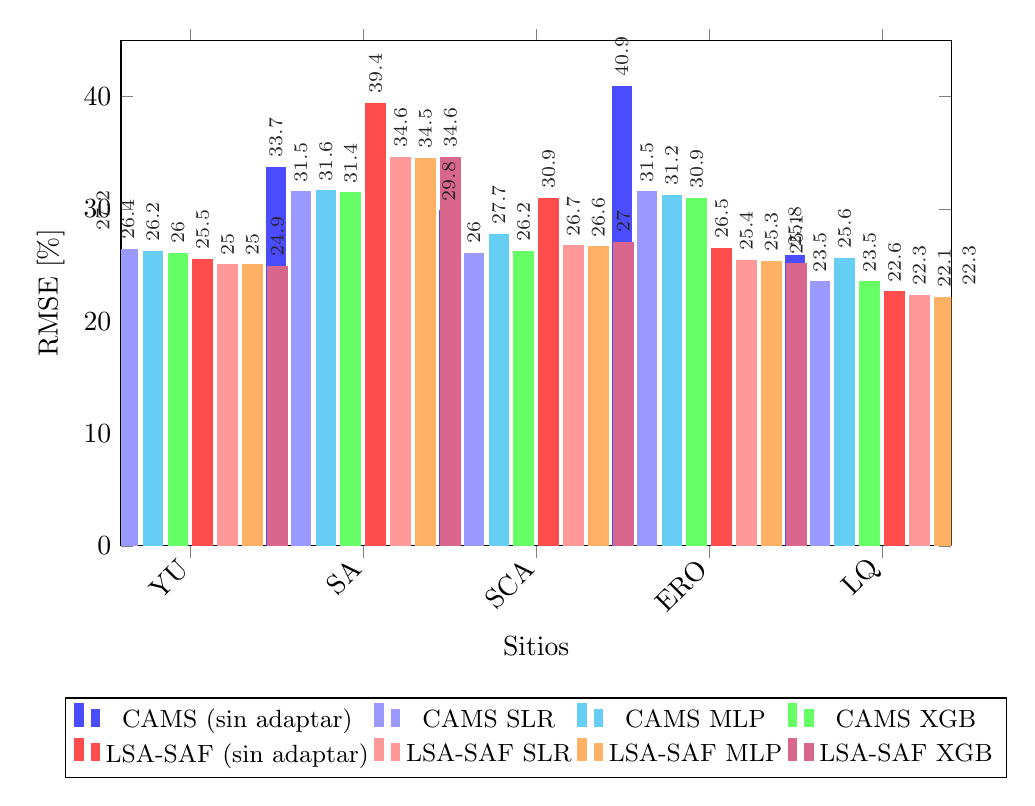
\begin{tikzpicture}
\begin{axis}[
    ybar,
    bar width=7pt,
    width=\linewidth,
    height=8cm,
    ylabel={RMSE [\%]},
    xlabel={Sitios},
    symbolic x coords={YU, SA, SCA, ERO, LQ},
    xtick=data,
    xticklabel style={rotate=45, anchor=east},
    enlarge x limits=0.1,
    ymin=0,
    nodes near coords,
    nodes near coords style={font=\scriptsize, rotate=90, anchor=west, text=black!85},
    legend style={at={(0.5,-0.30)}, anchor=north, legend columns=4, font=\small},
    cycle list={{blue!70},{blue!40},{cyan!60},{green!60},{red!70},{red!40},{orange!60},{purple!60}}
]

% ---- CAMS sin adaptar ----
\addplot+[fill=blue!70] coordinates {(YU,27.2) (SA,33.7) (SCA,29.8) (ERO,40.9) (LQ,25.8)};

% ---- CAMS adaptados ----
\addplot+[fill=blue!40] coordinates {(YU,26.4) (SA,31.5) (SCA,26.0) (ERO,31.5) (LQ,23.5)}; % SLR
\addplot+[fill=cyan!60] coordinates {(YU,26.2) (SA,31.6) (SCA,27.7) (ERO,31.2) (LQ,25.6)}; % MLP
\addplot+[fill=green!60] coordinates {(YU,26.0) (SA,31.4) (SCA,26.2) (ERO,30.9) (LQ,23.5)}; % XGB

% ---- LSA-SAF sin adaptar ----
\addplot+[fill=red!70] coordinates {(YU,25.5) (SA,39.4) (SCA,30.9) (ERO,26.5) (LQ,22.6)};

% ---- LSA-SAF adaptados ----
\addplot+[fill=red!40] coordinates {(YU,25.0) (SA,34.6) (SCA,26.7) (ERO,25.4) (LQ,22.3)}; % SLR
\addplot+[fill=orange!60] coordinates {(YU,25.0) (SA,34.5) (SCA,26.6) (ERO,25.3) (LQ,22.1)}; % MLP
\addplot+[fill=purple!60] coordinates {(YU,24.9) (SA,34.6) (SCA,27.0) (ERO,25.1) (LQ,22.3)}; % XGB

\legend{CAMS (sin adaptar), CAMS SLR, CAMS MLP, CAMS XGB, 
        LSA-SAF (sin adaptar), LSA-SAF SLR, LSA-SAF MLP, LSA-SAF XGB}
\end{axis}
\end{tikzpicture}
\caption{RMSE en resolución de 15 minutos para cada modelo y sitio, comparando modelos sin adaptación y adaptados.}
\label{fig:rmse15}
\end{figure}

La Figura \ref{fig:rmse15} muestra el comportamiento del RMSE (\%) en cada sitio para los diferentes modelos de regresión utilizados. Se observa que todas las propuestas de adaptación logran reducir el RMSE en cada sitio. Aunque en algunos casos la mejora puede ser modesta, como en YU y LQ, queda evidenciado que un simple ajuste específico puede mejorar el desempeño del modelo para una ubicación determinada. Además se puede apreciar que el grado de mejora mediante la adaptación aparenta depender del modelo de estimación empleado. Cada modelo impone un límite sobre la precisión de la serie resultante, y optimizar su salida no garantiza necesariamente un desempeño superior frente a otro modelo que, de forma natural, ya proporciona una estimación más adecuada para un sitio específico.\\




\begin{figure}
    \centering
    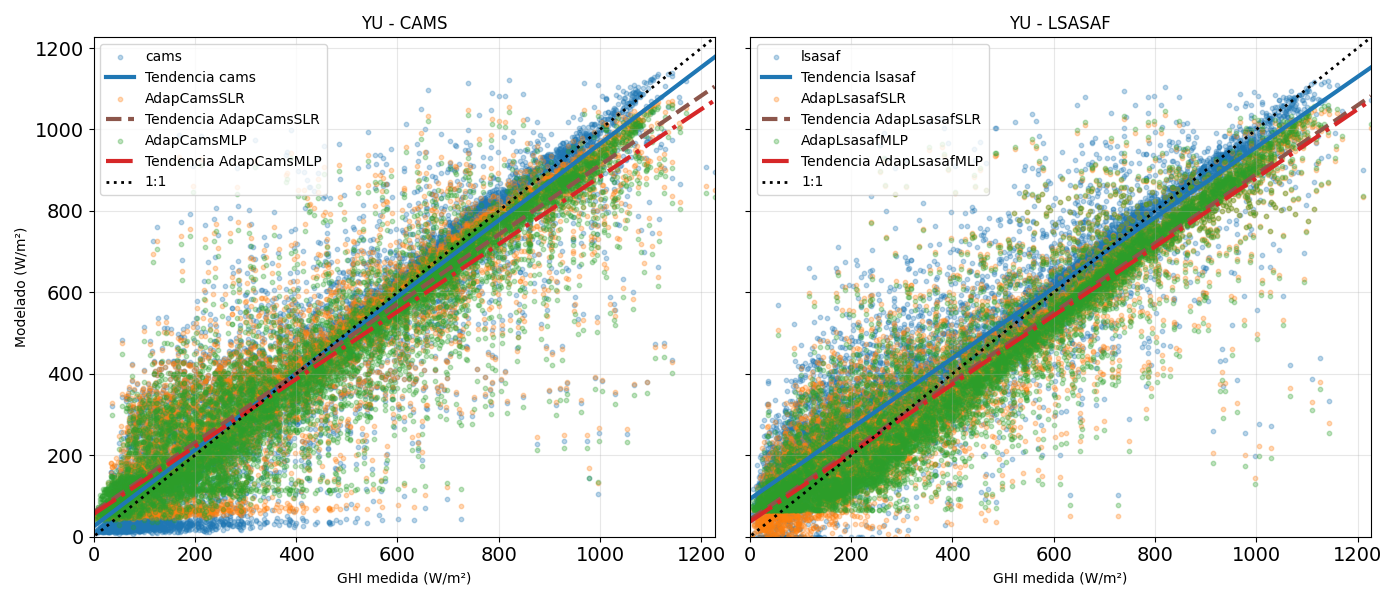
\includegraphics[width=0.9\textwidth]{figuras/scatter_yu_1.png}
    \caption{Comparación de modelos CAMS y LSASAF y las adpaciones con SLR y MLP en Yuto.}
    \label{fig:scatter-yu-01}
\end{figure}


La Figura \ref{fig:scatter-yu-01} muestra un gráfico de dispersión para la GHI medida y las los modelos de CAMS (izquierdo) y LSA-SAF (derecho) con sus correspondeintes adaptaciones usando SLR y MLP.   


\begin{figure}
    \centering
    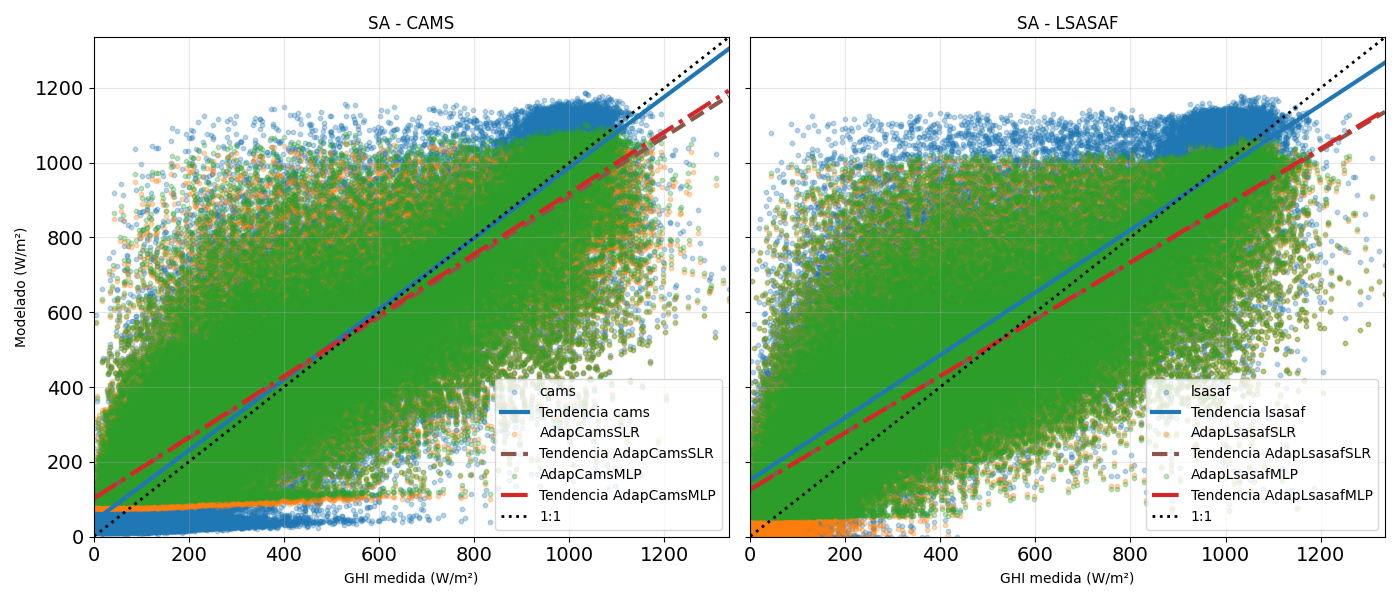
\includegraphics[width=0.9\textwidth]{figuras/scatter_sa_1.png}
    \caption{Comparación de modelos CAMS y LSASAF y las adaptaciones con SLR Y MLP en Salta.}
    \label{fig:scatter-sa-01}
\end{figure}


\begin{figure}
    \centering
    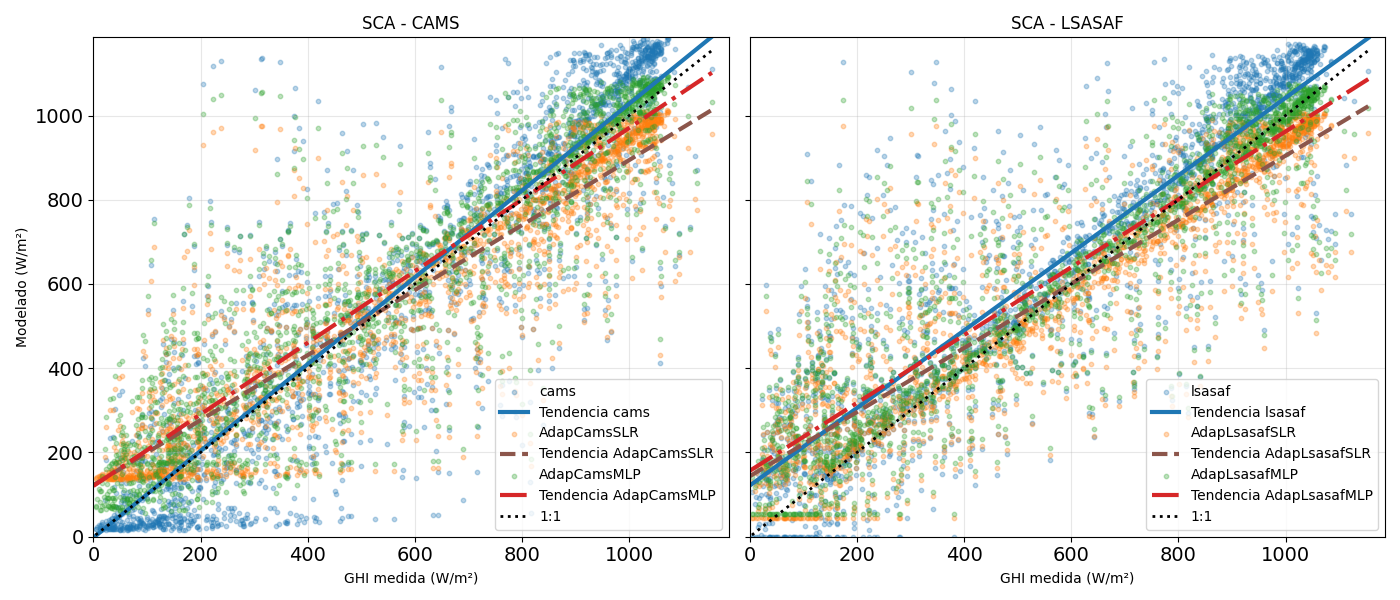
\includegraphics[width=0.9\textwidth]{figuras/scatter_sca_1.png}
    \caption{Comparación de modelos CAMS y LSASAF y las adpataciones con SLR y MLP en San Carlos.}
    \label{fig:scatter-sca-01}
\end{figure}


\begin{figure}
    \centering
    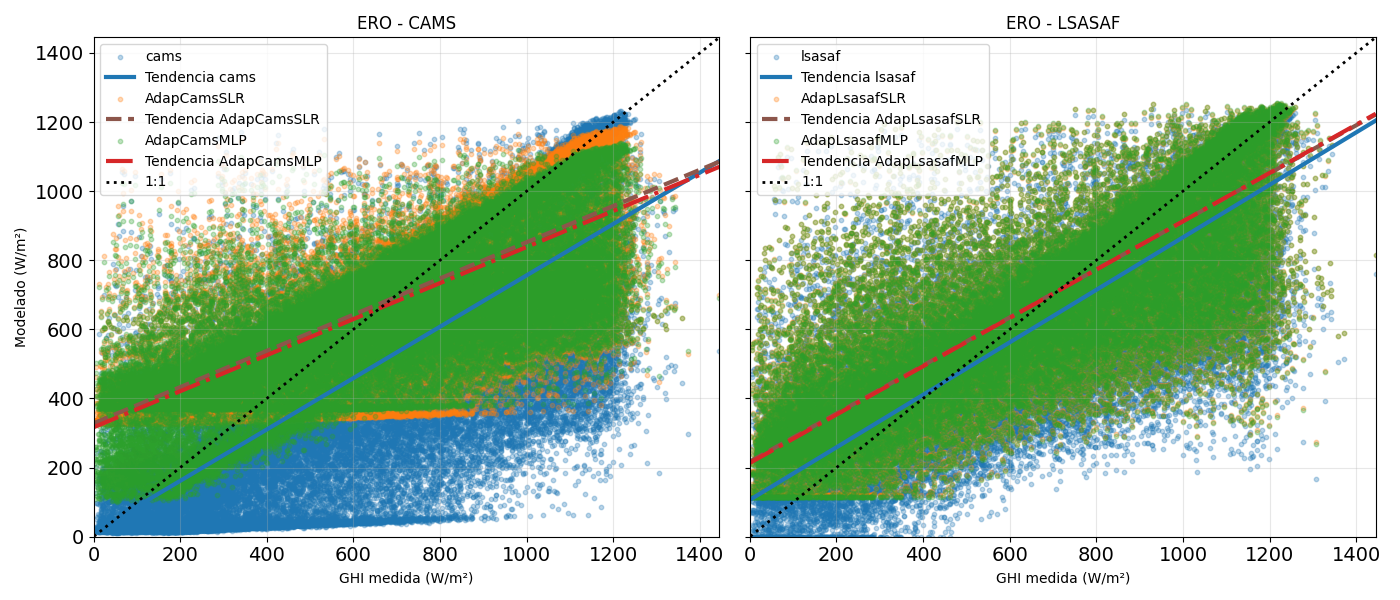
\includegraphics[width=0.9\textwidth]{figuras/scatter_ero_1.png}
    \caption{Comparación de modelos CAMS y LSASAF y las adaptaciones con SLR y MLP en El Rosal.}
    \label{fig:scatter-ero-01}
\end{figure}



\begin{figure}
    \centering
    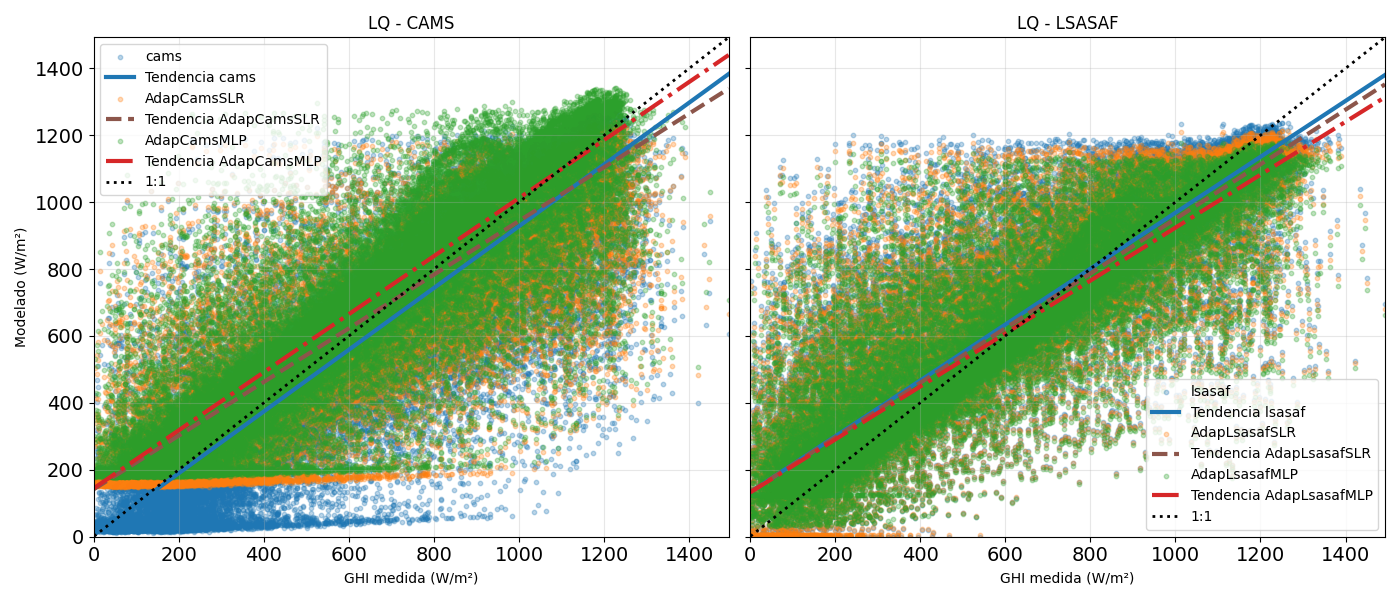
\includegraphics[width=0.9\textwidth]{figuras/scatter_lq_1.png}
    \caption{Comparación de modelos CAMS y LSASAF y las adaptaciones con SLR y MLP en La Quiaca.}
    \label{fig:scatter-lq-01}
\end{figure}



La Figura \ref{fig:mejorModelo} presenta las variaciones del rRMSE en cada sitio considerando el mejor desemepeño obtenido (menor rRMSE). Puede notarse que las ganancias sobre el desempeño podrían considerarse marginales, sin embargo sería interesante considerar el impacto que podria tener una variación del 3\% en la estimación del recurso solar, por ejemplo en la aplicación práctica.\\
\begin{figure}
    \centering
    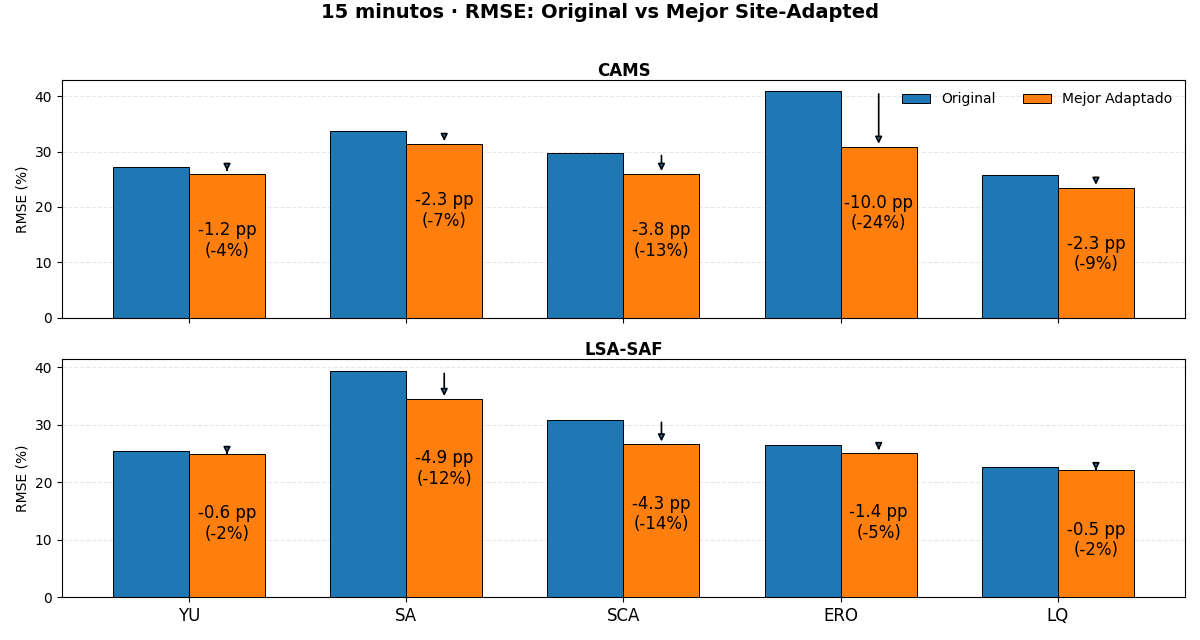
\includegraphics[width=0.9\textwidth]{figuras/comparativasRMSE15.png}
    \caption{Comparación del RMSE(\%) para los modelos crudos y el mejor desempeño obtenido.}
    \label{fig:mejorModelo}
\end{figure}





%\begin{figure}
%    \centering
%    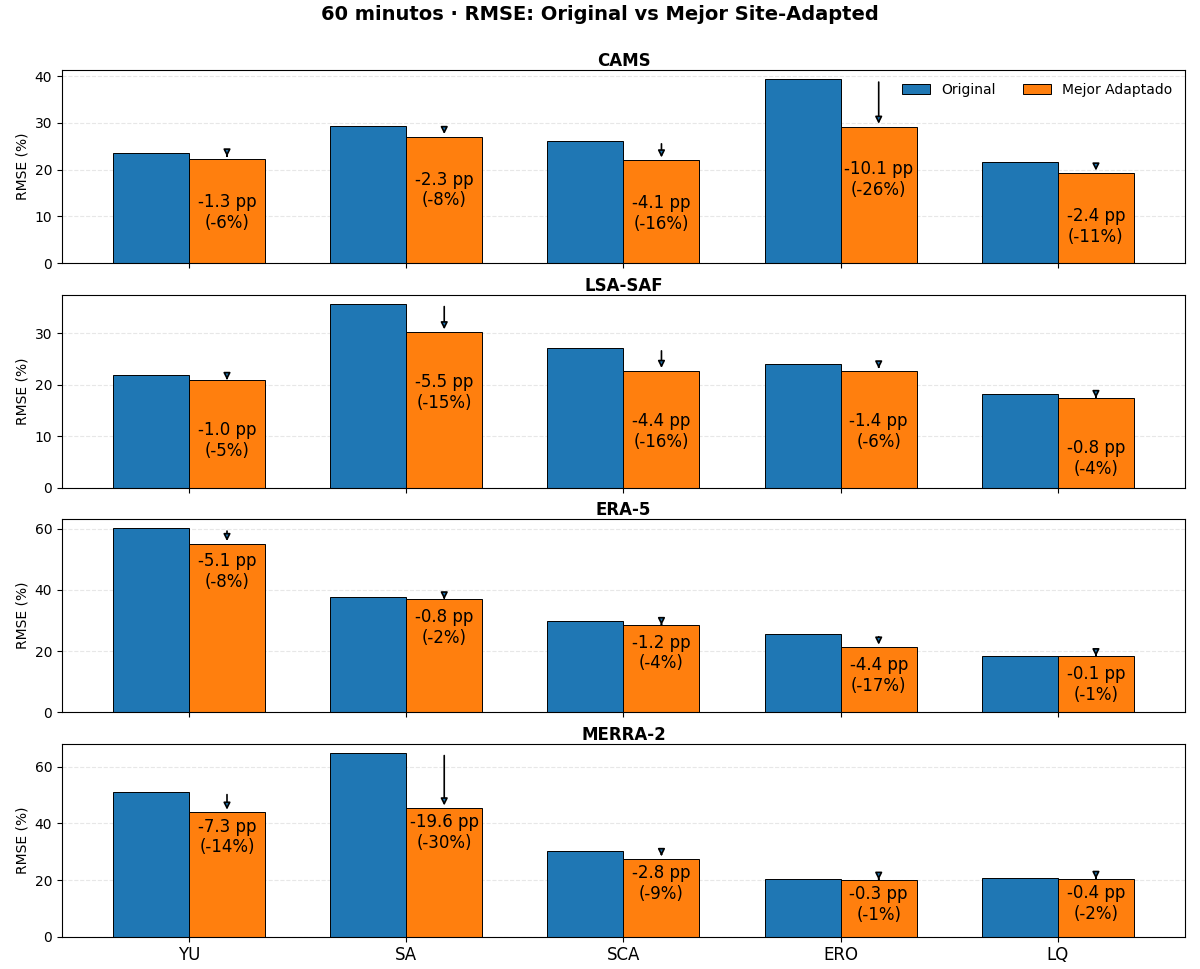
\includegraphics[width=0.9\textwidth]{figuras/comparativasRMSE60.png}
%    \caption{Variación del error cuadrático medio relativo (RRMSD) en función del ángulo cenital solar (SZA) para los cinco sitios analizados (YU, SA, SCA, ERO y LQ). Resultados para CAMS (líneas continuas) y LSASAF (líneas punteadas).}
%    \label{fig:RMSE-60}
%\end{figure}


Los hallazgos de este primer estudio indican que, en el contexto de la adaptación del sitio para GHI utilizando productos derivados de satélite como CAMS y LSA-SAF, los modelos de aprendizaje automático evaluados SLR, XGB y MLP mostraron un rendimiento comparable en términos de métricas de error estándar, con diferencias mínimas entre ellos. A pesar de su simplicidad, SLR demostró una notable capacidad para capturar la relación entre los datos derivados de satélite y las mediciones terrestres, logrando niveles de error relativo similares a los obtenidos por los modelos XGB y MLP, más complejos.
Estos resultados sugieren que la calidad de los datos de entrada impone un límite superior a las mejoras de precisión alcanzables que ofrecen los modelos complejos. Los productos satelitales empleados presentan incertidumbres inherentes y carecen de la resolución necesaria para considerar fenómenos localizados de alta frecuencia, como los efectos microclimáticos o la variabilidad inducida por el terreno. En consecuencia, aumentar la complejidad del modelo no mejora sustancialmente el rendimiento predictivo en estas condiciones de datos. En este sentido, la capacidad predictiva de los modelos complejos se vuelve redundante cuando la relación subyacente entre las variables es predominantemente lineal o solo ligeramente no lineal, lo que explica el excelente rendimiento del SLR.
Además, el análisis reveló que los modelos más flexibles, como el MLP, son propensos al sobreajuste, lo que genera un comportamiento inconsistente en diferentes métricas de rendimiento. Esto subraya la importancia de equilibrar la complejidad del modelo con la calidad de los datos para evitar comprometer la capacidad de generalización del modelo. En resumen, dada la calidad actual de los datos y las características del sitio, modelos simples como el SLR representan una solución robusta, interpretable y computacionalmente eficiente para la estimación del GHI adaptada al sitio. Es más probable lograr mejoras significativas en la precisión de la estimación incorporando variables meteorológicas adicionales, aplicando técnicas de descomposición temporal o desarrollando enfoques híbridos que combinen modelos físicos con correcciones estadísticas, en lugar de simplemente aumentar la complejidad de los algoritmos de aprendizaje automático.

 


\section{Adaptación al sitio con múltiples variables descriptivas}\label{sec:02}
En la sección anterior se presentaron los resultados del proceso de Adaptación al Sitio (SA) utilizando un enfoque basado en mejorar la estimación de un modelo a partir de la variable propiamente modelada y de mediciones in situ. Este enfoque tradicional se centra en la relación directa entre la variable objetivo y sus observaciones, pero en los últimos años se ha desarrollado una estrategia más avanzada que consiste en incorporar variables regresoras adicionales durante el entrenamiento de los modelos de regresión. La idea subyacente es que estas variables pueden aportar información complementaria, lo que podría mejorar la precisión de la estimación en comparación con un enfoque que utiliza únicamente una variable regresora. 

En la práctica, estas variables adicionales pueden provenir de distintos modelos de reanálisis o de fuentes satelitales, y se seleccionan con la expectativa de que estén correlacionadas, de alguna manera, con la irradiancia global horizontal (GHI) medida. Este enfoque ha sido aplicado y documentado en trabajos previos, como \cite{Salazar2025, Miranda2021, Miranda2023}.\\

La idea de ampliar el conjunto de regresores y automatizar el proceso de entrenamiento con la expectativa de obtener mejores resultados resulta atractiva, especialmente considerando que los modelos de aprendizaje automático son cada vez más utilizados para identificar patrones y extraer información de grandes volúmenes de datos. Sin embargo, la efectividad de estos modelos depende en gran medida de la calidad y relevancia de los regresores empleados. No basta con añadir más variables; estas deben ser apropiadas y contener información útil para la tarea de predicción.\\

En este contexto, la \textbf{selección de características} se convierte en un paso crítico del preprocesamiento de datos. Este proceso consiste en identificar las variables más relevantes y eliminar aquellas redundantes o irrelevantes \cite{liu2023, Huang2024}. La selección adecuada de características no solo incrementa la interpretabilidad del modelo, sino que también mejora su eficiencia computacional y su capacidad predictiva. Por el contrario, la inclusión de un exceso de variables o de regresores irrelevantes puede generar sobreajuste, donde el modelo muestra un buen desempeño en los datos de entrenamiento pero falla al generalizar a datos no vistos \cite{che2024a}. Al reducir la dimensionalidad y centrarse en las características más informativas, la selección de características fomenta la creación de modelos más robustos y generalizables, al tiempo que disminuye los costos computacionales y el tiempo requerido para entrenar el modelo, consolidándose como una herramienta esencial tanto para investigadores como para profesionales \cite{Cheng2024}.



Las técnicas de selección de características se agrupan en tres categorías principales: \textbf{métodos de filtro, métodos envolventes y métodos embebidos}, cada uno con su propia metodología, ventajas y limitaciones:  

\paragraph{Métodos de filtro.} Los métodos de filtro evalúan la relevancia de cada característica mediante criterios estadísticos como correlación, información mutua o varianza. Son computacionalmente eficientes y no dependen de un algoritmo de aprendizaje específico. Sin embargo, pueden no captar las interacciones entre variables. Ejemplos comunes incluyen la correlación de Pearson, las pruebas chi-cuadrado y la ganancia de información.  

\paragraph{Métodos envolventes.} Estos métodos consisten en entrenar y evaluar un modelo de aprendizaje automático múltiples veces para identificar el subconjunto óptimo de características. Técnicas como la selección hacia adelante, la eliminación hacia atrás y la eliminación recursiva de características (RFE) son ejemplos típicos \cite{Che2024b,liu2024}. Aunque suelen proporcionar mayor precisión, son costosos en términos computacionales y pueden no escalar eficientemente con conjuntos de datos grandes.  

\paragraph{Métodos embebidos.} Los métodos embebidos incorporan la selección de características directamente en el proceso de entrenamiento del modelo. Ejemplos incluyen técnicas de regularización como LASSO (regularización L1) y modelos basados en árboles de decisión. Este enfoque logra un equilibrio entre eficiencia y rendimiento, convirtiéndolo en una opción ampliamente utilizada en distintas aplicaciones. \\

Comprender estas técnicas permite a los profesionales seleccionar el método más adecuado según las características del conjunto de datos, el dominio del problema y las limitaciones computacionales.\\

En esta sección se documentan los resultados obtenidos al seleccionar tres métodos complementarios para la selección de variables con el objetivo de identificar los mejores regresores que contribuyan a la mejora de la estimación de la GHI en el contexto de la adaptación al sitio: RFE, LASSO y Stepwise.  

\paragraph{Eliminación recursiva de características (RFE).} RFE permite evaluar de manera iterativa la importancia de cada variable en el modelo, eliminando progresivamente las menos relevantes. Este enfoque es particularmente útil en el análisis de variables de geometría solar, donde pueden existir correlaciones complejas entre diferentes parámetros. Al utilizar RFE, se asegura que las variables seleccionadas aporten información significativa al modelo y reduzcan el riesgo de sobreajuste.  

\paragraph{LASSO (Least Absolute Shrinkage and Selection Operator).} LASSO integra la selección de variables en el propio proceso de entrenamiento mediante regularización L1. Este método penaliza los coeficientes de variables menos relevantes, promoviendo modelos más simples y generalizables. La utilización de LASSO en nuestro estudio permite manejar de manera eficiente la multicolinealidad entre parámetros solares y resaltar únicamente los regresores que contribuyen de manera significativa a la predicción de la GHI.  

\paragraph{Stepwise (selección hacia adelante y hacia atrás).} Los métodos Stepwise combinan criterios estadísticos de inclusión y exclusión de variables, permitiendo construir un modelo óptimo de manera secuencial. Este enfoque es especialmente adecuado cuando se busca un balance entre interpretabilidad y rendimiento predictivo. En el contexto de variables solares, Stepwise ayuda a identificar combinaciones de regresores que optimizan la estimación de la GHI sin introducir redundancias innecesarias. \\ 


La elección de los tres métodos de selección de variables se justifica por su complementariedad: RFE se centra en la importancia iterativa de cada predictor, LASSO introduce regularización para reducir la complejidad, y Stepwise optimiza la construcción del modelo desde un enfoque estadístico. Pretendemos que la combinación de estas técnicas permita una selección robusta de variables, maximizando la eficiencia del modelo.\\

En este trabajo el se propuso utilizar un conjunto de variables de carácter astronómico, atmosférico, satelital y meteorológico, definidas de la siguiente manera:

\begin{itemize}
\item \texttt{SZA}: Ángulo cenital solar.
\item \texttt{$\alpha$}: Altura solar.
\item \texttt{TOA}: Irradiancia en la parte superior de la atmósfera.
\item \texttt{GHIargp2}: Irradiancia bajo cielo despejado basada en \cite{Ledesma2023a}.
\item \texttt{delta}: Declinación solar.
\item \texttt{Fn}: Función normalizada de duración del día.
\item \texttt{E0}: Factor de corrección extraterrestre.
\item \texttt{mr}: Masa de aire relativa \cite{Gueymard2003}.
\item \texttt{tm}: Temperatura media del aire según ERA5.
\item \texttt{uw}: Componente U del viento según ERA5.
\item \texttt{dw}: Componente V del viento según ERA5.
\item \texttt{hr}: Humedad relativa según ERA5.
\item \texttt{p}: Presión según ERA5.
\end{itemize}


\begin{figure}
    \centering
    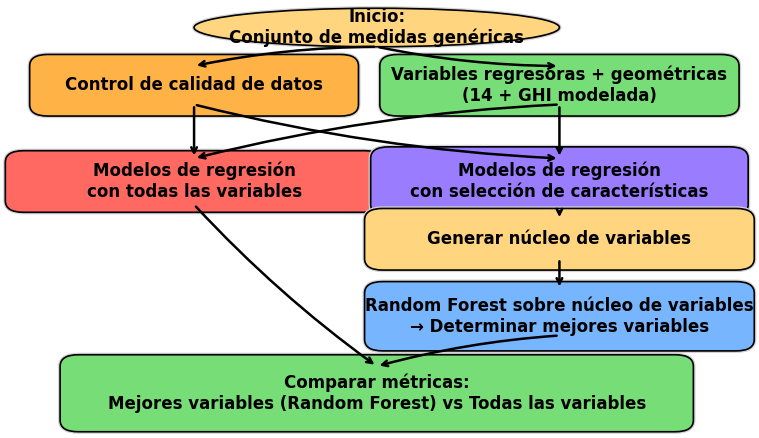
\includegraphics[width=0.65\textwidth]{figuras/procedure_1.png}
    \caption{Flujo de procesamiento para la adaptación de GHI en un sitio. A partir de un conjunto de medida, los datos pasan por un control de calidad y en paralelo se obtienen variables regresoras de reanálisis y geométricas. Con estas se entrenan modelos de regresión en dos enfoques: usando todas las variables disponibles o aplicando selección de características. El segundo enfoque genera un núcleo de variables que es refinado con Random Forest para identificar las más relevantes. Finalmente, se comparan las métricas de desempeño entre los modelos construidos con todas las variables y aquellos basados en las variables óptimas.}
    \label{fig:procedureSA01}
\end{figure}



Las métricas de desempeño obtenidas sobre las series generadas a partir del conjunto completo de variables regresoras se reporta en la Tabla \ref{tab:metricas_3_1}. Además se han incluido, para comidad del lector, nuevamente las métricas obtenidas en partir de la adaptación con una ùnica variable y sin adaptar.

\begin{table*}
\caption{Métricas de desempeño (MBE, MAE, RMSE) para cada modelo en el conjunto de prubeas de los cinco sitios. Los valores están normalizados y expresados como porcentajes relativos a la media de GHI en cada sitio: 429.2~W/m$^2$ (Yu), 432.9~W/m$^2$ (Sa), 554.4~W/m$^2$ (Sca), 628.4~W/m$^2$ (Ero), y 648.7~W/m$^2$ (Lq). Los modelos etiquetados con ``(1 var.)'' indican adaptación al sitio realizada utilizando solo un regresor (CAMS o LSA-SAF).}
\label{tab:metricas_3_1}
\centering
\resizebox{\linewidth}{!}{
\def\arraystretch{1.5}
\begin{tabular}{cccccccccccccccc}
\hline
      & \multicolumn{3}{c}{Yu} & \multicolumn{3}{c}{Sa} & \multicolumn{3}{c}{Sca} & \multicolumn{3}{c}{Ero} & \multicolumn{3}{c}{Lq} \\
Modelo & MBE & MAE & RMSE & MBE & MAE & RMSE  & MBE & MAE & RMSE & MBE & MAE & RMSE & MBE & MAE & RMSE  \\
\hline
\multicolumn{16}{|c|}{\textit{Estimaciones satelitales en bruto}} \\
\hline
CAMS    & -0.2 & 17.4 & 27.2 &  3.9 & 23.4 & 33.7 &  2.6 & 21.8 & 29.8 & -23.6 & 27.6 & 40.9 & -6.9 & 16.5 & 25.8 \\
LSA-SAF &  7.6 & 16.5 & 25.5 & 17.9 & 27.4 & 39.4 & 13.1 & 22.2 & 30.9 &  -7.7 & 16.2 & 26.5 &  4.0 & 12.6 & 22.6 \\
\hline

\multicolumn{16}{|c|}{\textit{Adaptación al sitio con un solo regresor (1 var.)}} \\
\hline
SLR-CAMS    & -0.9 & 17.1 & 26.4 &  3.8 & 21.3 & 31.5 & -1.5 & 18.4 & 26.0 &  2.5 & 24.8 & 31.5 &  2.1 & 15.9 & 23.5 \\
XGB-CAMS (1 var.) & -1.3 & 17.1 & 26.0 &  3.8 & 21.4 & 31.4 & -1.8 & 18.9 & 26.2 &  2.5 & 23.9 & 30.9 &  2.2 & 15.9 & 23.5 \\
MLP-CAMS (1 var.) & -4.4 & 17.7 & 26.2 &  4.8 & 21.4 & 31.6 &  7.7 & 17.8 & 27.7 &  0.5 & 24.1 & 31.2 &  9.1 & 19.4 & 25.6 \\
SLR-LSASAF  & -5.5 & 18.4 & 25.0 &  4.4 & 23.9 & 34.6 &  1.0 & 18.0 & 26.7 &  2.7 & 17.1 & 25.4 &  2.2 & 12.9 & 22.3 \\
XGB-LSASAF (1 var.) & -6.0 & 18.2 & 24.9 &  4.3 & 23.9 & 34.6 &  0.5 & 18.6 & 27.0 &  2.4 & 17.2 & 25.1 &  2.3 & 13.1 & 22.3 \\
MLP-LSASAF (1 var.) & -7.1 & 18.6 & 25.0 &  4.5 & 23.6 & 34.5 &  5.9 & 18.4 & 26.6 &  2.5 & 17.0 & 25.3 & -0.4 & 13.6 & 22.1 \\
\hline
\multicolumn{16}{|c|}{\textit{Adaptación al sitio con 15 regresores}} \\
\hline
MLR-CAMS    & -4.1 & 17.2 & 25.5 &  3.7 & 21.0 & 31.1 &  0.7 & 18.9 & 27.0 &  0.6 & 14.4 & 22.3 &  3.8 & 12.9 & 21.2 \\
XGB-CAMS    & -3.5 & 16.5 & 24.6 &  3.4 & 20.5 & 30.6 & -1.5 & 19.9 & 27.5 &  0.4 & 13.9 & 22.5 &  2.1 & 12.9 & 21.7 \\
MLP-CAMS    & -2.8 & 17.2 & 25.5 &  0.8 & 20.5 & 30.8 &  1.2 & 17.6 & 26.3 & -0.7 & 14.7 & 23.2 &  2.1 & 13.4 & 21.8 \\
MLR-LSASAF  & -5.5 & 16.9 & 24.5 &  4.0 & 23.8 & 34.0 & -0.2 & 20.9 & 28.5 &  0.9 & 13.5 & 21.6 &  1.6 & 13.1 & 21.6 \\
XGB-LSASAF  & -5.3 & 16.9 & 24.1 &  3.9 & 23.4 & 33.8 & -1.2 & 22.5 & 30.6 &  0.8 & 13.1 & 21.7 &  1.9 & 13.6 & 22.8 \\
MLP-LSASAF  & -4.0 & 18.5 & 25.7 &  3.8 & 23.5 & 34.7 & -4.2 & 22.0 & 29.4 & -2.0 & 14.4 & 22.3 &  1.5 & 14.0 & 22.3 \\

\hline

\hline
\end{tabular}}
\end{table*}


La Tabla \ref{tab:metricas_3_1} permite ver que al incorporar los 15 regresores, los MLR y XGB logran una mejora adicional en MAE y RMSE en casi todos los sitios. En contraste, en las evaluaciones de MLP con muchas variables se experimenta un aumento de los errores en varios sitios en comparación a los demás modelos de regresión. Incluso empeorando la estimación origanl de los modelos. Debe tenerse en cuenta que a pesar de implementar un esquema de entrenamiento con conjunto de entrenamiento, validación y prueba (TVT) y aplicar early stopping para evitar sobreajuste, los modelos MLP aparentan tener un desempeño inferior al esperado cuando se incluyen múltiples variables regresoras. Esto se debe a que las redes neuronales dependen de que las entradas contengan información relevante y no redundante; si algunas variables son irrelevantes el modelo podría aprender patrones espurios, lo que incrementa métricas como MAE o RMSE. En este contexto, incluso estrategias de regularización y control de complejidad solo limitan parcialmente la degradación del desempeño. Por ello, la selección cuidadosa de variables mediante técnicas como RFE, LASSO o Stepwise resulta crucial para garantizar que los MLP aprovechen su capacidad de modelar relaciones no lineales sin comprometer la precisión de la estimación de la GHI.\\


Seguido de esto aplicamos los mismos algoritmos (MLR, MLP, XGBoost) después de reducir las variables mediante tres técnicas complementarias de selección: Eliminación Recursiva de Variables (RFE), LASSO y selección Stepwise. Estas metodologías se emplearon de manera conjunta, ya que ofrecen distintas perspectivas sobre la relevancia de las variables: RFE mediante eliminación iterativa, LASSO a través de regularización incorporada, y Stepwise basándose en criterios estadísticos. A nuestro criterio ninguna de estas técnicas por sí sola podría denifir un conjunto de variables a considerar óptimas, pero su uso combinado nos permitió identificar un conjunto central consistente de variables relevantes, reduciendo la complejidad del modelo sin comprometer su capacidad predictiva.\\

El análisis comparativo de los métodos de selección a lo largo de los sitios estudiados (YU, SA, SCA, ERO y LQ) reveló que Stepwise generalmente ofreció el mejor desempeño, con la menor desviación cuadrática media relativa (\textit{rrmsd}). Por ejemplo, en ERO y LQ los errores se aproximaron al 21\%, mientras que en YU y SCA oscilaron entre 25–27\%. Esto sugiere que la inclusión progresiva únicamente de aquellos predictores que mejoran significativamente el ajuste proporciona un equilibrio más efectivo que la eliminación exhaustiva (RFE) o la penalización intensa (LASSO).

En a las series de GHI, los resultados, nuevamente podrían indicarnos que no existe una fuente superior de manera universal: la elección entre CAMS y LSA-SAF depende del sitio específico. En YU y ERO, los modelos basados en LSA-SAF mostraron menores errores, mientras que en SCA y LQ CAMS presentó un mejor desempeño. En SA, sin embargo, ambos productos mostraron un rendimiento inferior (\textit{rrmsd} entre 31\% y 34\%), probablemente esto indique que SA presenta condiciones locales más complejas en comparación a los otros sitios lo que introduce limitaciones en los resultados de los modelos de satélite.\\

Respecto a la composición de los predictores, la variable GHI derivada de satélites (\texttt{cams} o \texttt{lsasaf}) se incluyó de manera consistente en todos los modelos, confirmando su rol central. De igual manera, variables geométricas como el ángulo cenital solar (\texttt{SZA}), ángulo horario (\texttt{w}), día del año (\texttt{N}) e índice de claridad (\texttt{kt}) aparecieron recurrentemente en las configuraciones de mejor desempeño. Otras variables astronómicas y meteorológicas, incluyendo \texttt{TOA}, \texttt{GHIargp2}, temperatura del aire (\texttt{tm}) y componentes del viento (\texttt{uw}, \texttt{vw}), fueron seleccionadas con frecuencia, reforzando la importancia de integrar tanto la geometría solar como las condiciones meteorológicas locales. Por el contrario, variables como \texttt{Fn}, \texttt{delta}, \texttt{alphaS}, \texttt{E0} y \texttt{mr} fueron menos elegidas, indicando una contribución más dependiente del sitio.\\

En términos generales, el análisis conduce a las siguientes conclusiones:
\begin{itemize}
\item La selección Stepwise constituye la estrategia de selección de variables más efectiva, equilibrando precisión y complejidad.
\item La fuente satelital óptima depende del sitio: LSA-SAF es favorable en YU y ERO, mientras que CAMS funciona mejor en SCA y LQ.
\item Los predictores astronómicos y meteorológicos complementan los regresores basados en satélite y mejoran significativamente el desempeño del modelo.
\item Las variables derivadas de ERA5 (\texttt{tm}, \texttt{uw}, \texttt{vw}) aportan beneficios adicionales, especialmente en sitios donde los productos satelitales presentan un desempeño inferior.
\item Las diferencias específicas por sitio son significativas: ERO y LQ muestran el mejor desempeño (\textit{rrmsd} $\approx$ 21\%), YU y SCA presentan resultados intermedios (25–27\%), mientras que SA registra los mayores errores (>31\%).
\end{itemize}

A partir de este análisis, se puede identificar un conjunto central de predictores consistentemente relevantes: {N,; w,; TOA,; kt,; SZA,; GHIargp2,; \text{cams/lsasaf},; tm,; uw,; vw}. Este conjunto combina predictores con sólida fundamentación física y selección recurrente, ofreciendo un equilibrio robusto entre generalización y adaptabilidad específica por sitio. Variables secundarias como \texttt{Fn}, \texttt{delta}, \texttt{alphaS}, \texttt{E0} y \texttt{mr} aún pueden contribuir en contextos particulares.\

Es importante señalar, no obstante, que RFE, LASSO y Stepwise no producen rankings explícitos de importancia de las variables. Sus resultados deben interpretarse en función de la frecuencia y consistencia con la que los predictores son seleccionados a lo largo de sitios y métodos. Para complementar esta limitación, se empleó posteriormente Random Forest como modelo de regresión, con hiperparámetros optimizados mediante búsqueda en malla (Tabla~T). Más allá de su función predictiva, RF proporciona un ranking directo de importancia de los regresores. Aunque estudios previos \cite{SALAMALIKIS2022} han demostrado que XGBoost generalmente supera a RF en tareas de adaptación por sitio, el ranking obtenido con RF sigue siendo valioso para optimizar costo computacional y tiempo de entrenamiento en aplicaciones futuras. El ranking de importancia resultante se presenta en la Tabla \ref{tab:rf_importance}.\\


\begin{table}[t]
\centering
\caption{Predictores mejor posicionados según el análisis de importancia de Random Forest en los distintos sitios y fuentes satelitales (CAMS, LSA-SAF). Los valores representan puntuaciones de importancia normalizadas.}
\label{tab:rf_importance}
\resizebox{\linewidth}{!}{
\begin{tabular}{lcccccc}
\toprule
\textbf{Sitio} & \textbf{Fuente} & \textbf{1°} & \textbf{2°} & \textbf{3°} & \textbf{4°} & \textbf{5°} \\
\midrule
YU & CAMS & cams (0.310) & kt (0.193) & SZA (0.080) & GHIargp2 (0.070) & alphaS (0.069) \\
YU & LSA-SAF & lsasaf (0.296) & kt (0.214) & SZA (0.078) & GHIargp2 (0.068) & alphaS (0.063) \\
SA & CAMS & cams (0.276) & kt (0.198) & SZA (0.096) & mr (0.076) & alphaS (0.073) \\
SA & LSA-SAF & lsasaf (0.274) & kt (0.130) & SZA (0.106) & mr (0.100) & alphaS (0.072) \\
SCA & CAMS & cams (0.674) & TOA (0.054) & GHIargp2 (0.047)& alphaS (0.035) & tm (0.026) \\
SCA & LSA-SAF & lsasaf (0.682) & alphaS (0.055) & GHIargp2 (0.029)& tm (0.029) & w (0.028) \\
ERO & CAMS & alphaS (0.388) & SZA (0.158) & mr (0.158) & cams (0.052) & tm (0.034) \\
ERO & LSA-SAF & alphaS (0.351) & SZA (0.149) & mr (0.143) & lsasaf (0.141) & N (0.030) \\
LQ & CAMS & cams (0.208) & SZA (0.145) & alphaS (0.141) & mr (0.134) & GHIargp2 (0.108) \\
LQ & LSA-SAF & lsasaf (0.246) & SZA (0.177) & mr (0.146) & alphaS (0.143) & GHIargp2 (0.094) \\
\bottomrule
\end{tabular}}
\end{table}


Los rankings de importancia obtenidos con RF evidencian tanto patrones comunes como diferencias específicas por sitio. En todos los casos, el predictor derivado de satélite (\texttt{cams} o \texttt{lsasaf}) apareció de manera consistente entre las variables mejor clasificadas, confirmando su rol central en la estimación de GHI. Predictores complementarios como el índice de claridad (\texttt{kt}), el ángulo cenital solar (\texttt{SZA}) y variables astronómicas auxiliares (p. ej., \texttt{alphaS}, \texttt{mr}, y \texttt{TOA}) también recibieron puntuaciones de importancia elevadas de manera recurrente, reforzando la conclusión de que la combinación de entradas satelitales con geometría solar mejora la robustez del modelo.\\

A pesar de esta estructura común, los rankings revelaron dependencias marcadas por sitio. Por ejemplo, en SCA la variable satelital dominó el ranking, representando más del 67\% de la importancia total, lo que indica una fuerte dependencia del GHI derivado de satélite en este sitio. En contraste, en ERO los predictores principales fueron variables angulares (\texttt{alphaS}, \texttt{SZA}, \texttt{mr}), con la contribución del satélite inferior al 15\%, destacando el papel de la geometría solar bajo condiciones locales. En LQ, la importancia se distribuyó de manera más equilibrada entre satélite (\texttt{cams}/\texttt{lsasaf}), variables angulares y factores atmosféricos, reflejando una contribución balanceada de los predictores.\\

Las variables meteorológicas de ERA5, como la temperatura del aire (\texttt{tm}) y los componentes del viento (\texttt{uw}, \texttt{vw}), aparecieron consistentemente en posiciones medias o bajas del ranking. Aunque su contribución relativa fue menor en comparación con las variables satelitales y geométricas, su selección recurrente sugiere que aportan poder explicativo complementario, especialmente en sitios donde los productos satelitales presentan menor desempeño (p. ej., SA).\\

En conjunto, los rankings de RF refuerzan las conclusiones obtenidas a partir de los métodos de selección: (i) el GHI derivado de satélite es indispensable, (ii) las variables geométricas son recurrentemente importantes en todos los sitios, (iii) los predictores atmosféricos agregan mejoras dependientes del sitio, y (iv) la contribución relativa de cada familia de predictores varía considerablemente según la ubicación. Esta variabilidad específica por sitio confirma la importancia de adaptar los modelos de regresión no solo a la fuente de datos disponible, sino también a las condiciones locales predominantes.\\


\begin{table*}[ht!]
\caption{Métricas de desempeño (MBE, MAE, RMSE) para cada modelo y conjunto satelital en los cinco sitios, utilizando los siete predictores mejor posicionados con resolución de 15 minutos. Los valores están normalizados y expresados como porcentaje respecto al GHI promedio de cada sitio: 429.2~W/m$^2$ (YU), 432.9~W/m$^2$ (SA), 554.4~W/m$^2$ (SCA), 628.4~W/m$^2$ (ERO) y 648.7~W/m$^2$ (LQ).}
\label{tab:metrics_7pred}
\centering
\resizebox{\linewidth}{!}{
\def\arraystretch{1.5}
\begin{tabular}{cccccccccccccccc}
\hline
& \multicolumn{3}{c}{YU} & \multicolumn{3}{c}{SA} & \multicolumn{3}{c}{SCA} & \multicolumn{3}{c}{ERO} & \multicolumn{3}{c}{LQ} \\
Modelo & MBE & MAE & RMSE & MBE & MAE & RMSE & MBE & MAE & RMSE & MBE & MAE & RMSE & MBE & MAE & RMSE \\
\hline
\multicolumn{16}{|c|}{\textit{Adaptación por sitio con 7 regresores}} \\
\hline
MLR-CAMS & -1.6 & 17.1 & 25.9 & 4.1 & 20.9 & 31.1 & 1.5 & 18.5 & 26.8 & 1.0 & 14.3 & 22.3 & 4.5 & 12.8 & 21.4 \\
MLP-CAMS & 1.4 & 16.4 & 24.8 & 1.5 & 20.5 & 30.9 & 0.6 & 18.0 & 25.8 & 0.5 & 13.6 & 22.0 & 2.9 & 12.9 & 21.3 \\
XGB-CAMS & -1.7 & 16.9 & 25.6 & 4.0 & 20.8 & 31.3 & 0.0 & 19.0 & 26.5 & 0.3 & 13.6 & 22.1 & 2.5 & 12.6 & 21.2 \\
MLR-LSA-SAF & -4.9 & 17.1 & 24.6 & 4.5 & 23.4 & 34.3 & 2.2 & 19.8 & 28.3 & 1.6 & 13.4 & 21.8 & 6.4 & 13.2 & 23.1 \\
MLP-LSA-SAF & -5.7 & 16.5 & 24.4 & 4.8 & 22.9 & 34.1 & 2.4 & 20.2 & 28.8 & -0.5 & 13.3 & 21.4 & 3.0 & 13.2 & 21.8 \\
XGB-LSA-SAF & -5.0 & 16.6 & 24.2 & 4.2 & 23.8 & 34.4 & 1.8 & 20.0 & 28.6 & 0.8 & 12.7 & 21.5 & 2.2 & 13.2 & 21.9 \\
\hline
\end{tabular}}
\end{table*}



\begin{figure}
    \centering
    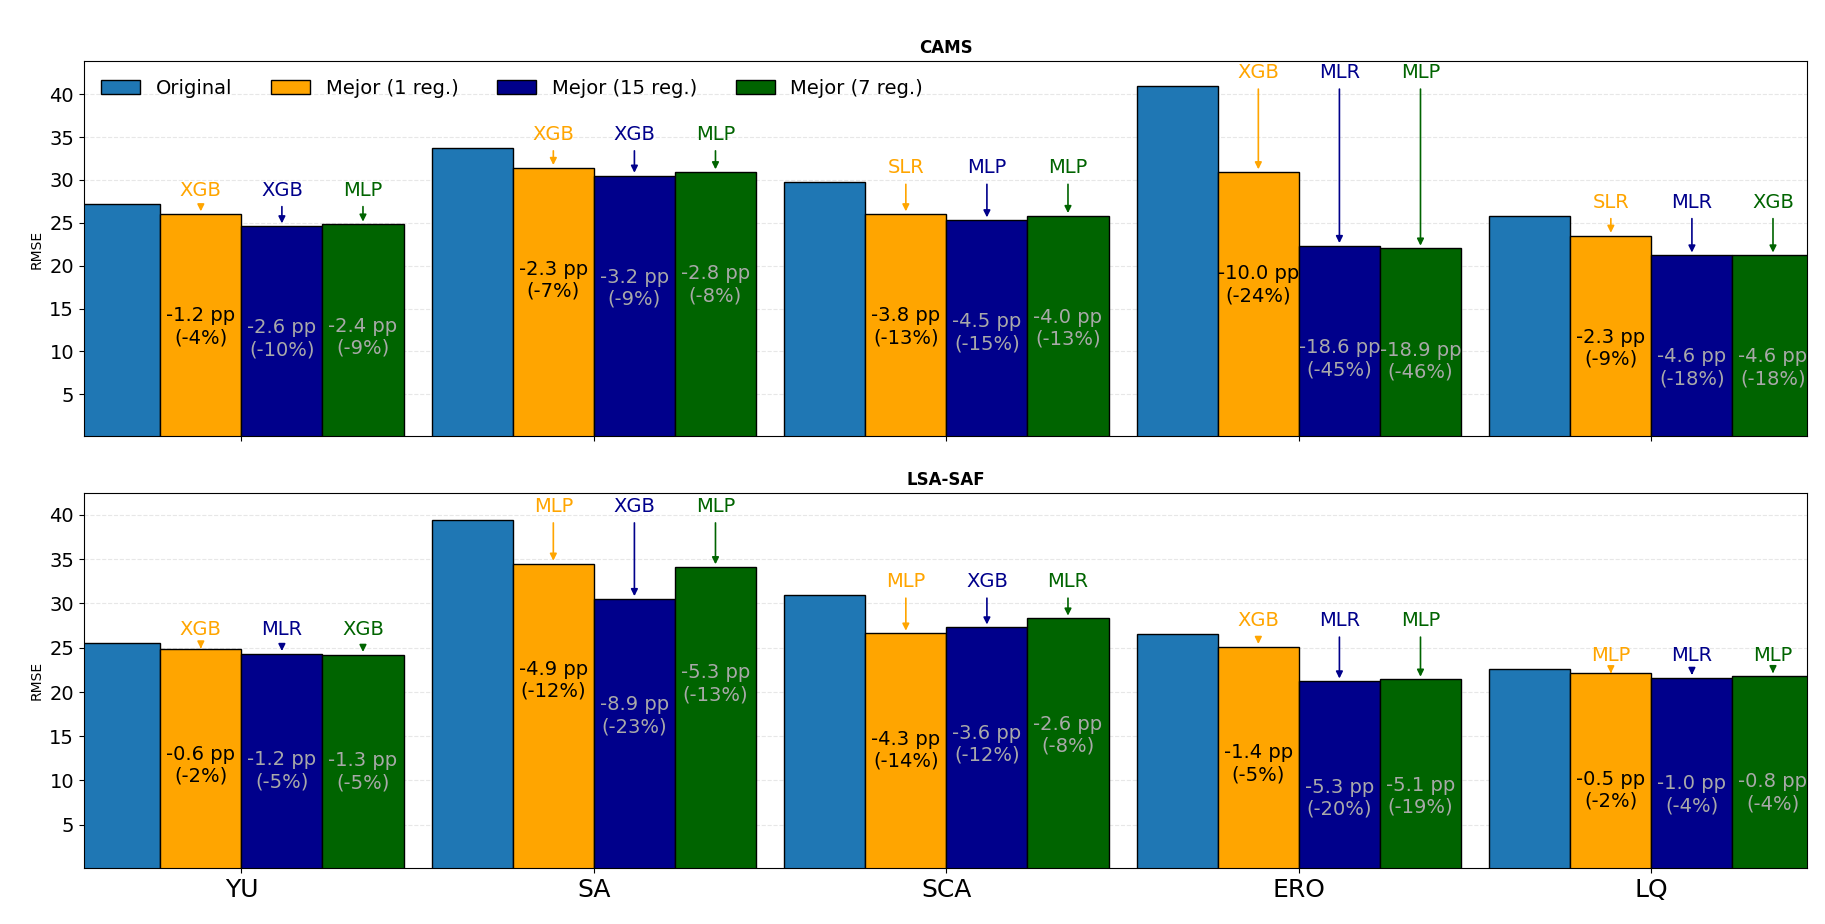
\includegraphics[width=\textwidth]{figuras/rmsd-multiple-mejor.png}
    \caption{Comparación del rendimiento entre el modelo original y los modelos ajustados con 15, 7 y 1 regresor en términos de RMSD. Las barras se muestran agrupadas por sitio y conjunto de datos, junto con flechas que indican la mejora o el deterioro con respecto al modelo original, así como deltas en puntos porcentuales (pp) y porcentaje relativo.}
    \label{fig:rrmsd-multiple}
\end{figure}


La Figura \ref{fig:rrmsd-multiple} muestra que incluso ante el mejor resultado que se puede obtener usando un conjunto amplio de variables regresoras se puede obtener un desempeño similar si toman algunas consideraciones sobre qué variables van a introducirse como fuentes descriptivas al modelo de regresiòn.\\



Por otro lado, pensamos que la selección de siete predictores representa un compromiso adecuado entre la simplicidad del modelo y su capacidad predictiva. Este subconjunto fue elegido considerando tanto los rankings de importancia de variables como los resultados de los análisis de selección de características, lo que permite capturar de manera consistente los factores que más influyen en la variabilidad del GHI, al tiempo que se minimiza la redundancia. La utilización de siete regresores facilita la retención de información clave proveniente de fuentes satelitales y meteorológicas, permitiendo una adaptación precisa por sitio sin incurrir en un elevado costo computacional. Como se observa en la Tabla~\ref{tab:metrics_7pred}, los modelos que emplean este conjunto de variables presentan valores de MAE entre 12 y 20\% y RMSE en el rango de 21–31\% del GHI promedio, lo que indica que un conjunto compacto puede ofrecer un desempeño comparable al de configuraciones más extensas, a la vez que mejora la interpretabilidad y la eficiencia del entrenamiento. No obstante, es importante reconocer que un análisis más profundo podría evaluar el impacto de reducir aún más el número de variables, especialmente en términos de precisión y generalización del modelo.\\









\section{Adaptación al sitio usando celdas satelitáles adyacentes al sitio de interés}
En las Secciones \ref{sec:01} y \ref{sec:02} se han presentado las primeras evaluaciones del proceso de adaptación al sitio en la región del NOA, siguiendo enfoques previamente reportados en la literatura por distintos autores. Las implementaciones basadas en estos enfoques nos han proporcionado una base sólida para comprender la influencia del entorno local en la variable GHI, además hemos dimesionado cuales son los límites en la mejora que se puede obtener tras site adaptar una serie siguiendo estos enfoques.\\


Las evaluaciones realizadas en este trabajo y en estudios previos sobre SA se han basado exclusivamente en datos medidos en una estación meteorológica. Estos datos se combinan con una o más variables modeladas —provenientes de una celda satelital o de un modelo de reanálisis— que representan geográficamente la ubicación de dicha estación. En otras palabras, la información utilizada para entrenar y validar los modelos de corrección se limita a la celda específica del punto de medición, sin considerar el contexto espacial más amplio que podría aportar información adicional relevante.\\

Los enfoques previos de SA aplicados a mediciones terrestres de una estación enfrentan una limitación intrínseca: la información derivada de los productos satelitales es finita, lo que restringe la capacidad de aprendizaje de cualquier técnica de aprendizaje automático implementada, incluso sin sobreajuste. Para superar esta restricción, proponemos un enfoque que amplía el alcance espacial de los datos de entrada incorporando valores de GHI modelados de celdas satelitales adyacentes. La hipótesis central es que la variabilidad de la irradiancia solar en un punto no es aislada, sino que forma parte de una estructura espacialmente coherente gobernada por la dinámica atmosférica regional. Al incluir las estimaciones de irradiancia de celdas vecinas como predictores adicionales, el modelo dispone de información espacial más rica, mejorando su capacidad para identificar patrones complejos y generalizar de manera más efectiva.\\

Este enfoque busca aprovechar correlaciones bien documentadas en los campos de irradiancia solar, impulsadas por el movimiento de nubes, el transporte de aerosoles y los sistemas meteorológicos a escala sinóptica \citep{IHSAN2024}. A diferencia de los métodos tradicionales de AS, que se limitan a variables locales dentro de una sola celda, el marco propuesto utiliza de manera innovadora la irradiancia satelital de las celdas circundantes como características de entrada para los modelos de aprendizaje automático. Hasta ahora, ningún trabajo había explorado explícitamente esta integración del contexto espacial.\\


\begin{figure}
    \centering
    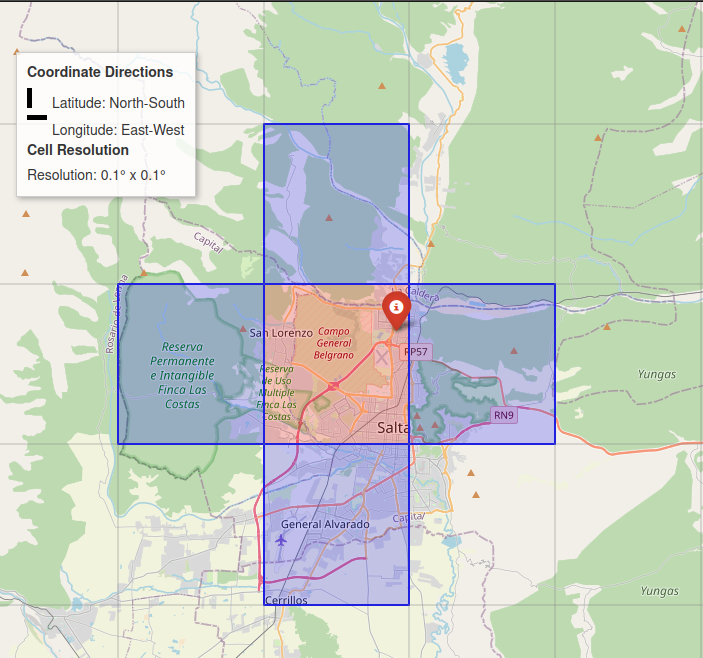
\includegraphics[width=0.7\textwidth]{figuras/gridSA.png}
    \caption{Grilla utilizada por el modelo Helisat-4 de CAMS distribuido por CAMS Volume}
    \label{fig:gridSA}
\end{figure}

Este enfoque asume que las celdas adyacentes \ref{fig:gridSA} están sujetas a condiciones atmosféricas similares —particularmente la cobertura de nubes— que la celda central. Dada la resolución espacial de los productos satelitales (~16 km para CAMS), es razonable esperar que los valores de GHI en las celdas vecinas estén altamente correlacionados con aquellos medidos en la celda que contiene la estación en tierra. Además, considerando que, para cualquier producto de radiación de servicios como CAMS, LSA-SAF, ERA5 o MERRA-2, el GHI modelado suele ser la variable más correlacionada con el GHI observado, tiene sentido elegir este producto como base para la adaptación al sitio y la incorporación de regresores espaciales adicionales que capturen la variabilidad local.

La adaptación propuesta integra estos regresores distribuidos espacialmente dentro del marco de aprendizaje automático. El valor adaptado de GHI se estima como:

\begin{equation}
GHI_{adaptado} = ML_{Regresor}(GHI_{modelado}, X_{ij}),
\label{ec:SiteAdap}
\end{equation}

\noindent donde $ML_{Regresor}$ denota un modelo de aprendizaje automático entrenado con el conjunto de datos, $GHI_{modelado}$ es el GHI modelado perteneciente a algùn servicio (CAMS, LSA-SAF, etc) en el sitio de interés, y $X_{ij}$ representa los valores de GHI de las celdas circundantes obtenidos del producto correspondiente.

La selección de celdas vecinas se basa en la distancia Manhattan (MD), definida como:

\begin{equation}
DM = \frac{|\text{lat}p - \text{lat}{ac}|}{\Delta} + \frac{|\text{lon}p - \text{lon}{ac}|}{\Delta},
\label{ec:dist}
\end{equation}

\noindent donde $\Delta$ es la resolución de la grilla, $(lat_{p}, lon_{p})$ denota las coordenadas geográficas del punto de interés, y $(lat_{ac}, lon_{ac})$ corresponde a las coordenadas de una celda vecina (adyacente).

La MD permite identificar automáticamente las celdas satelitales adyacentes que rodean la celda central donde se encuentra la estación en tierra. Consideramos que esta métrica es adecuada porque, los productos de los servicios de estimación están organizados en una cuadrícula regular de latitud–longitud, formando una malla rectangular. En dicha grilla, las celdas se alinean en filas y columnas, y la MD, definida como la suma de las diferencias absolutas en latitud y longitud normalizadas por la resolución de la grilla, captura efectivamente el número de pasos necesarios para alcanzar una celda vecina tanto horizontal como verticalmente.

Las celdas con $DM=1$ son directamente adyacentes a la celda central (es decir, al norte, sur, este u oeste), siendo las más relevantes para capturar la variabilidad espacial local de las condiciones atmosféricas. A diferencia de la distancia euclidiana, que enfatiza la proximidad radial, la MD refleja mejor las relaciones de vecindad en productos satelitales en grilla, asegurando que la información espacial utilizada para la adaptación site-specific sea consistente con la estructura regular del producto.

En conjunto, esta metodología permite que la adaptación del GHI al sitio integre tanto la estimación directa del producto satelital como la información de celdas vecinas, mejorando la capacidad de predicción local y la transferencia del modelo a diferentes condiciones espaciales.



\begin{table*}%[]
  \centering
  \label{tab:metrics-as-4}
  \caption{Métricas de desempeño (MBE, MAE, RMSE) para cada modelo adaptado en los cinco sitios en el \textbf{conjunto de pruebas}}
  \resizebox{\linewidth}{!}{%
    \begin{tabular}{|l|ccc|ccc|ccc|ccc|ccc|}
      \hline
      & \multicolumn{3}{c|}{YU} & \multicolumn{3}{c|}{SA} & \multicolumn{3}{c|}{SCA} & \multicolumn{3}{c|}{ERO} & \multicolumn{3}{c|}{LQ} \\
      \cline{2-16}
      Modelo  & MBE & MAE & RMSE & MBE & MAE & RMSE & MBE & MAE & RMSE & MBE & MAE & RMSE & MBE & MAE & RMSE \\
      \hline
      \multicolumn{16}{|c|}{\textit{Resolución Temporal: 15 minutos}} \\
      \hline
      LSA-SAF MLR     & -5  & 16.5 & 24.6 & 3.2 & 23.8 & 35.2 & -2.9 & 18.5 & 25.7 & 1.4 & 12.8 & 21.4 & 2.8 & 12.7  & 21.7\\ 
      LSA-SAF MLP     & -6  & 16.4 & 24.3 & 1.9 & 23.2 & 35.3 & 1.3  & 16.7 & 25.3 & 2   & 12.5 & 21.4  & 4.7 & 12.6 & 21.7\\       
      \hline
      \multicolumn{16}{|c|}{\textit{Resolución Temporal: horaria}} \\
      \hline
      LSA-SAF MLR    & 5.6 & 14.8 & 21.2 & 2.6 & 21.5 & 31.9 & -3.8 & 16.6 & 22.4 & 1.9 & 11.3 & 18.8 & 0.2 & 10.4 & 16.8\\ 
      ERA5 MLR       & 1.8 & 22.8 & 33.7 & 7   & 26.5 & 36.8 & -2.2 & 19.5 & 26.2 & 1.1 & 10.7 & 17.8 & 0.9 & 10.4 & 16.7\\
      ERA5 MLP       &-2.3 & 23.1 & 33.3 & -0.4 & 27.6 & 36.5 & -2.1 & 19.6 & 26   & -0.7& 11.9 & 18.4 & 1.5 & 10.9 & 17.5 \\
      \hline
      
      \hline	
    \end{tabular}%
  }
\end{table*}


Resulta de gran interés analizar el comportamiento de los modelos de regresión cuando se aplican en sitios distintos de aquellos en los que fueron entrenados. A este enfoque vamos a denominarlo validación cruzada entre sitios.\\

Este procedimiento consiste en entrenar un modelo en un sitio determinado y posteriormente evaluar su desempeño en otros sitios geográficamente diferentes. De esta manera, es posible analizar la capacidad de generalización espacial del modelo, es decir, su habilidad para mantener un rendimiento aceptable fuera del entorno en el que fue ajustado originalmente.\

La validación cruzada entre sitios permite evaluar si las correcciones o ajustes aplicados en un sitio pueden extenderse a un territorio más amplio. Esto resulta especialmente útil para el desarrollo de mapas o modelos regionales adaptados a sitios.\\

\begin{figure}
\centering
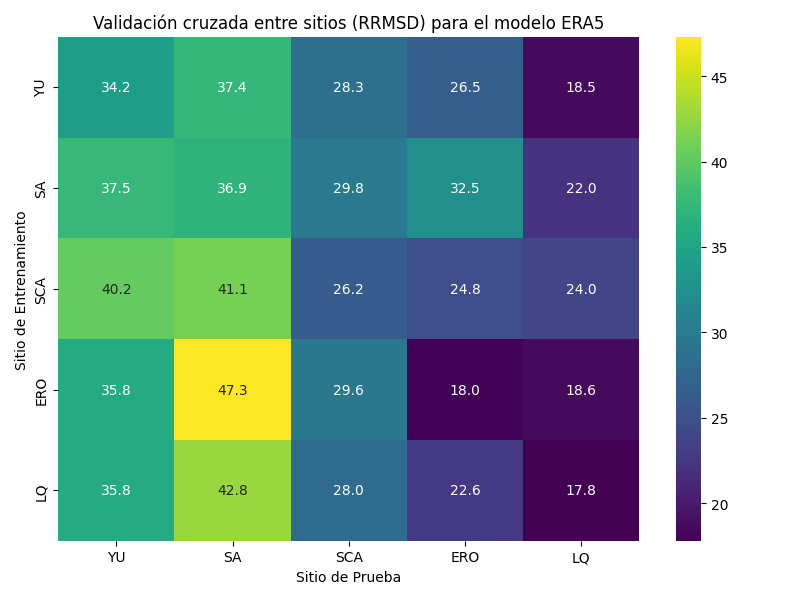
\includegraphics[width=0.7\textwidth]{figuras/CrossValidationOneSite.png}
\caption{Matriz de rRMSD (\%) obtenida a partir de la validación cruzada entre sitios para el modelo ERA5, utilizando los modelos ajustados con celdas satelitales adyacentes al sitio de interés.}
\label{fig:crossValidation}
\end{figure}

La Figura \ref{fig:crossValidation} muestra un análisis de sensibilidad en función del rRMSD (\%) obtenido a partir de las validaciones cruzadas realizadas en cada sitio para ERA5 utilizando los MLP ajustados, siguiendo el enfoque de adaptación al sitio presentado anteriormente en esta sección.


\begin{figure}
\centering
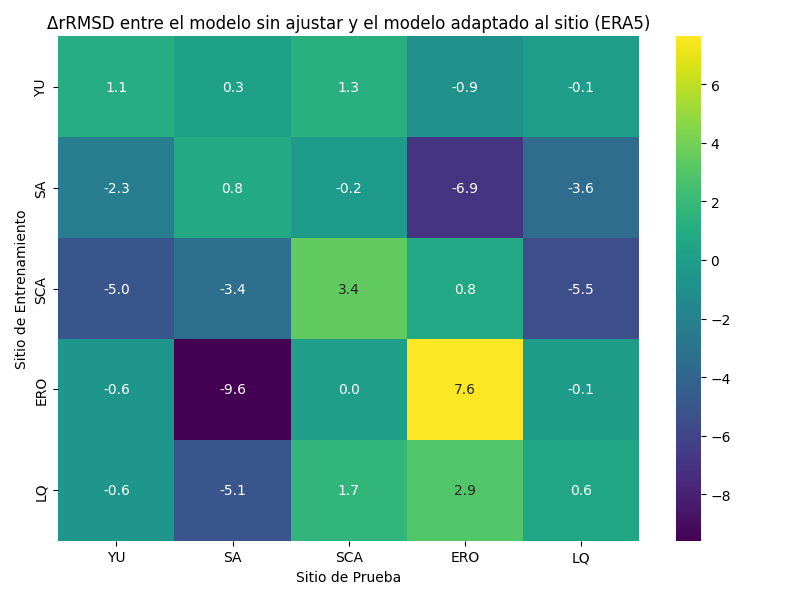
\includegraphics[width=0.7\textwidth]{figuras/DeltaCrossValidationOneSite.png}
\caption{Diferencia en desempeño entre el modelo sin ajustar (ERA5 original) y el modelo adaptado a cada sitio. Cada fila indica el sitio de entrenamiento y cada columna el sitio de prueba.}
\label{fig:deltaCrossValidation}
\end{figure}


La Figura \ref{fig:deltaCrossValidation} muestra la matriz de diferencias del rRMSD
($\Delta \text{rRMSD} = \text{rRMSD}_{\text{ERA5 original}} - \text{rRMSD}_{\text{site-adapted}}$) 
para los cinco sitios considerados: YU (401 m), SA (1230 m), SCA (1320 m), ERO (3355 m) y LQ (3500 m). 
Cada fila representa el sitio de entrenamiento y cada columna el sitio de prueba.

Los valores positivos indican que la adaptación al sitio reduce el error respecto al modelo ERA5 sin ajustar, mientras que los valores negativos muestran un empeoramiento. Se pueden destacar varias tendencias relevantes:

\begin{itemize}
    \item \textbf{Mejoras locales dominantes:} La diagonal de la matriz muestra que los modelos entrenados en un sitio específico obtienen la mayor reducción de rRMSD en el mismo sitio, evidenciando la eficacia de la adaptación local. Por ejemplo, el modelo entrenado en ERO reduce el error en 7.63\% al evaluarse en ERO, y el modelo de YU mejora 1.1\% en YU.
    
    \item \textbf{Influencia de la altitud:} Los modelos entrenados en sitios de baja altitud (YU) tienden a degradar el desempeño en sitios de alta montaña (ERO, LQ), mientras que los modelos entrenados en altitudes elevadas (ERO, LQ) no generalizan bien hacia sitios bajos. Esto resalta que la altitud es un factor determinante en la radiación solar y, por ende, en la capacidad de generalización de los modelos.
    
    \item \textbf{Transferencia entre sitios de altitud similar:} Los modelos entrenados en altitudes medias (SA, SCA) presentan mejoras moderadas cuando se aplican a sitios cercanos en altitud, pero no funcionan bien en extremos altitudinales. Esto indica que la transferencia espacial es más efectiva entre sitios con condiciones físicas y climáticas semejantes.
    
    \item \textbf{Robustez espacial limitada:} Si bien la adaptación al sitio mejora notablemente el desempeño local, los valores negativos fuera de la diagonal muestran que la generalización a sitios lejanos o con gran diferencia altitudinal puede ser limitada. Este resultado es consistente con la influencia de la nubosidad, elevación y ángulo solar en la radiación incidente.
\end{itemize}


En función del desempeño obtenido en la validación cruzada, podemos concluir que la transferencia de un modelo ajustado a otro sitio no es automática. Para la construcción de mapas \emph{site-adapted} a escala regional, a partir de este análisis se podrían considerar las siguientes alternativas:

\begin{enumerate}
    \item Entrenar modelos representativos para distintos rangos de altitud.
    \item Agrupar sitios con características climáticas y altitudinales similares para mejorar la transferencia del modelo.
    \item Evitar la aplicación directa de modelos entrenados en sitios bajos hacia sitios de alta montaña sin ajuste, debido al riesgo de degradar el desempeño.
\end{enumerate}




\section{Adaptación al sitio tomando consideraciones de una serie temporal}


En la presente sección se introducen los resultados obtenidos al aplicar un enfoque exploratorio desarrollado en esta tesis, basado en la desestacionalización de series temporales, con el objetivo de mejorar el proceso de adaptación al sitio (AS).

Una serie temporal se define como un conjunto de observaciones de una o más variables recolectadas y ordenadas cronológicamente. El orden temporal no es arbitrario, sino que es esencial para el análisis, la interpretación y la modelización de los datos, ya que permite identificar patrones, tendencias y comportamientos periódicos que pueden ser fundamentales para la toma de decisiones \cite{Olivas2022}.

El análisis de series temporales tiene aplicaciones en múltiples disciplinas. En Economía, permite estudiar la evolución de precios, la demanda de productos o la inflación. En Marketing, facilita la comprensión de la dinámica de ventas a lo largo del tiempo. En Medicina, las bioseñales, como el electrocardiograma (ECG), el electroencefalograma (EEG) o el electrooculograma (EOG), son ejemplos claros de series temporales utilizadas para diagnóstico y monitoreo de pacientes. Además, en la gestión hospitalaria, el análisis temporal puede aplicarse para evaluar la afluencia de pacientes a servicios de urgencias o la demanda de especialistas en diferentes períodos. Otro ámbito crucial es la meteorología, que constituye el foco principal de este trabajo. En este contexto, las series temporales permiten caracterizar, clasificar y predecir variables climáticas de interés, como la irradiancia global horizontal (GHI), entre otras.

Una característica clave de muchas series temporales es la estacionalidad, que se manifiesta cuando los datos muestran fluctuaciones regulares y predecibles con una frecuencia constante. Esta frecuencia puede ser diaria, semanal, mensual o anual, dependiendo del fenómeno que se estudie. Por ejemplo, en meteorología, la GHI presenta variaciones estacionales debidas a cambios en la posición del sol, la nubosidad o las condiciones atmosféricas. La presencia de estacionalidad puede influir significativamente en la interpretación y modelización de los datos, dado que introduce patrones repetitivos que podrían enmascarar otras tendencias o variaciones importantes.

El enfoque propuesto en esta tesis consiste en desestacionalizar las series temporales de GHI antes de aplicar el proceso de adaptación al sitio. La desestacionalización implica eliminar o ajustar estas fluctuaciones periódicas, de manera que se pueda analizar la serie en términos de su comportamiento subyacente, sin que las variaciones estacionales interfieran en la evaluación del proceso de AS. Este procedimiento permite comparar los datos en condiciones más homogéneas, mejorando la precisión y confiabilidad de los análisis.

En esta sección se evalúa el impacto de considerar la estacionalidad en la serie GHI sobre el proceso de AS, comparando el enfoque tradicional, que no realiza ajustes, con una metodología propuesta de desestacionalización.


En el proceso de \textbf{SA tradicional}, si consideramos como modelo de regresión al método \textbf{SLR}, que es el más simple de los distintos modelos disponibles, podemos expresar el proceso mediante la siguiente ecuación:

\begin{equation}
GHI_{\text{adaptada}} = a \cdot GHI_{\text{modelada}} + b,
\label{ec:approache1}
\end{equation}

donde \(GHI_{\text{adaptada}}\) representa la irradiancia global horizontal ajustada, \(GHI_{\text{modelada}}\) es la irradiancia modelada (por estimación satelital o re-análisis), y \(a\) y \(b\) son los coeficientes de regresión lineal, a este enfoque de ahora en más vamos a llamarlo Enfoque 1.\\

El Enfoque 2 se basa en la estrategia propuesta por \cite{ZAINALI2024}. En este enfoque, la variable regresora es el GHI modelado ($GHI_{\text{modelado}}$), y la variable objetivo se define como la diferencia entre el GHI medido y el modelado, es decir, 
$\Delta_{GHI} = GHI_{\text{medido}} - GHI_{\text{modelado}}$. Una vez obtenida la variable objetivo, el GHI adaptado se recupera sumando el factor de error $\Delta_{GHI}$ al GHI modelado.

\begin{align}
\Delta_{GHI} &= GHI_{\text{medido}} - GHI_{\text{modelado}} \\
GHI_{\text{adaptado}} &= GHI_{\text{modelado}} + (a \cdot \Delta_{GHI} + b)
\label{eq:approach2}
\end{align}


En este enfoque, la variable regresora se define como la diferencia entre el GHI modelado desestacionalizado, que se obtiene restando el GHI de cielo despejado del GHI modelado ($GHI_{\text{modelado}} - GHI_{\text{cielo despejado}}$). La variable objetivo corresponde a la diferencia entre el GHI medido desestacionalizado y el GHI de cielo despejado ($GHI_{\text{medido}} - GHI_{\text{cielo despejado}}$). Una vez estimada la variable objetivo, el valor corregido del GHI se recupera sumando nuevamente el GHI de cielo despejado.

\begin{align}
X &= GHI_{\text{modelado}} - GHI_{\text{cielo despejado}} \\
Y &= GHI_{\text{medido}} - GHI_{\text{cielo despejado}} \\
GHI_{\text{adaptado}} &= GHI_{\text{cielo despejado}} + (a \cdot X + b)
\label{eq:approach3}
\end{align}

En cada caso, los coeficientes $a$ y $b$ se obtienen mediante regresión lineal simple. El modelo de GHI de cielo despejado utilizado en este estudio es el modelo ARGP-V2 \cite{Ledesma2023a}.

\begin{figure*}[ht!]
\centering
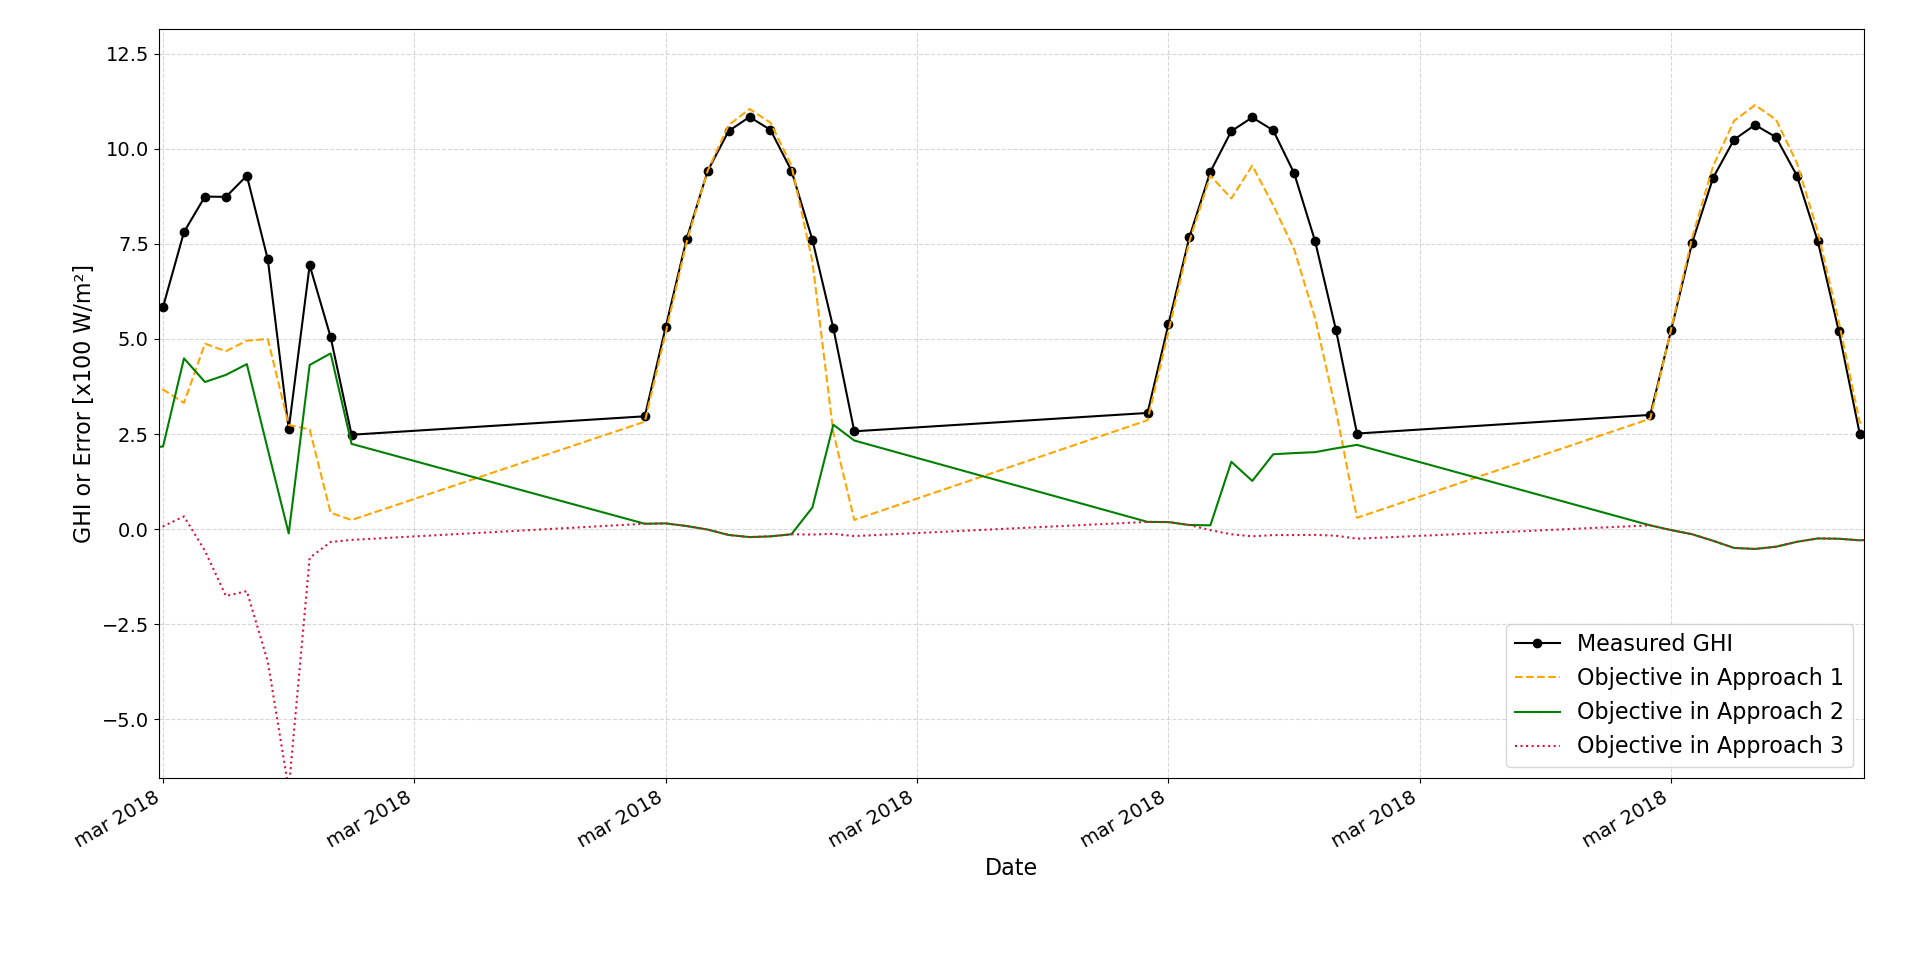
\includegraphics[width=\textwidth]{figuras/approaches.png}
\caption{Diferencias entre los tres enfoques de adaptación.}
\label{fig:approaches}
\end{figure*}



Los resultados obtenidos para cada uno de estos enfoques se presentan en la Tabla T. Cabe destacar que el Enfoque 1 fue es el evaluado en las secciones anteriores en esta tesis; para facilitar una comparación, se ha incluido también el reporte de las métricas correspondientes a este enfoque.




\begin{table*}
\caption{Métricas de desempeño (MBE, MAE, RMSE) para cada modelo en el conjunto de prubeas de los cinco sitios. Los valores están normalizados y expresados como porcentajes relativos a la media de GHI en cada sitio: 429.2~W/m$^2$ (Yu), 432.9~W/m$^2$ (Sa), 554.4~W/m$^2$ (Sca), 628.4~W/m$^2$ (Ero), y 648.7~W/m$^2$ (Lq). Los modelos etiquetados con ``(1 var.)'' indican adaptación al sitio realizada utilizando solo un regresor (CAMS o LSA-SAF).}
\label{tab:metricas_4_1}
\centering
\resizebox{\linewidth}{!}{
\def\arraystretch{1.5}
\begin{tabular}{cccccccccccccccc}
\hline
      & \multicolumn{3}{c}{Yu} & \multicolumn{3}{c}{Sa} & \multicolumn{3}{c}{Sca} & \multicolumn{3}{c}{Ero} & \multicolumn{3}{c}{Lq} \\
Modelo & MBE & MAE & RMSE & MBE & MAE & RMSE  & MBE & MAE & RMSE & MBE & MAE & RMSE & MBE & MAE & RMSE  \\
\hline
\multicolumn{16}{|c|}{\textit{Estimaciones satelitales en bruto}} \\
\hline
CAMS    & -0.2 & 17.4 & 27.2 &  3.9 & 23.4 & 33.7 &  2.6 & 21.8 & 29.8 & -23.6 & 27.6 & 40.9 & -6.9 & 16.5 & 25.8 \\
LSA-SAF &  7.6 & 16.5 & 25.5 & 17.9 & 27.4 & 39.4 & 13.1 & 22.2 & 30.9 &  -7.7 & 16.2 & 26.5 &  4.0 & 12.6 & 22.6 \\
\hline
\multicolumn{16}{|c|}{\textit{Adaptación al sitio usando Enfoque 1 (E1)}} \\
\hline
SLR-CAMS    & -0.9 & 17.1 & 26.4 &  3.8 & 21.3 & 31.5 & -1.5 & 18.4 & 26.0 & 2.5 & 24.8 & 31.5 & 2.1 & 15.9 & 23.5 \\
SLR-LSASAF  & -5.5 & 18.4 & 25.0 &  4.4 & 23.9 & 34.6 &  1.0 & 18.0 & 26.7 & 2.7 & 17.1 & 25.4 & 2.2 & 12.9 & 22.3 \\
\hline
\multicolumn{16}{|c|}{\textit{Adaptación al sitio usando Enfoque 2 (E2)}} \\
\hline
SLR-CAMS    & -0.9 & 17.1 & 26.4 &  3.8 & 21.3 & 31.5 & -1.5 & 18.4 & 25.9 & 2.5 & 24.8 & 31.5 & 2.1 & 15.9 & 23.5 \\
SLR-LSASAF  & -5.5 & 18.4 & 25   &  4.4 & 23.9 & 34.6 &  1   & 18   & 26.7 & 2.7 & 17.1 & 25.4 & 2.2 & 12.8 & 22.3 \\
\hline
\multicolumn{16}{|c|}{\textit{Adaptación al sitio usando Enfoque 3 (E3)}} \\
\hline
SLR-CAMS    & -2   & 17.5 & 27.1 &  3.8 & 22.7 & 33.3 & 3.3 & 19.1 & 28.6 & 0.1 & 13.6 & 22   & 2.9 & 12.7 & 21.2 \\
SLR-LSASAF  & -5.3 & 16.7 & 24.7 &  4.2 & 23.8 & 35.4 & 4.3 & 19.2 & 28.7 & 0.9 & 12.7 & 21.5 & 2.6 & 12.8 & 21.9  \\
\hline
\end{tabular}}
\end{table*}


La Tabla \ref{tab:metricas_4_1} y la Figura \ref{fig:metricas_estacionalidad} muestran las métricas de desempeño obtenidas tras evaluar los tres enfoques sobre la desestacionalización de la serie. Se comparan las estimaciones satelitales originales (CAMS y LSA-SAF) con sus adaptaciones al sitio mediante los enfoques E1, E2 y E3. 
Cada subplot corresponde a una métrica distinta, y dentro de cada sitio se presentan primero los modelos basados en CAMS y luego, separados visualmente, los basados en LSA-SAF. 

El Enfoque 1, que aplica una regresión lineal simple sobre los valores modelados, tiende a funcionar de manera consistente cuando la relación entre la irradiancia modelada y la medida es aproximadamente lineal y estable a lo largo del tiempo. Sin embargo, puede ser menos efectivo en sitios donde existen patrones estacionales complejos o variaciones sistemáticas que no se capturan con una regresión simple. 

El Enfoque 2, basado en modelar la diferencia entre el GHI medido y el modelado, permite ajustar directamente el error sistemático y suele mejorar el desempeño en sitios donde el sesgo del modelo es relativamente constante, pero puede fallar si las diferencias presentan fuerte dependencia estacional o si los errores son heterocedásticos a lo largo del año.

Finalmente, el Enfoque 3, que desestacionaliza tanto la variable regresora como la objetivo usando el GHI de cielo despejado, permite capturar patrones estacionales más complejos y corregir errores dependientes del ciclo solar diario y anual. Esto explica por qué, en general, presenta mejores métricas de rMAE y rRMSE en sitios con alta variabilidad estacional, como Ero y Lq, donde los enfoques anteriores muestran limitaciones.\\





\begin{figure}
    \centering
    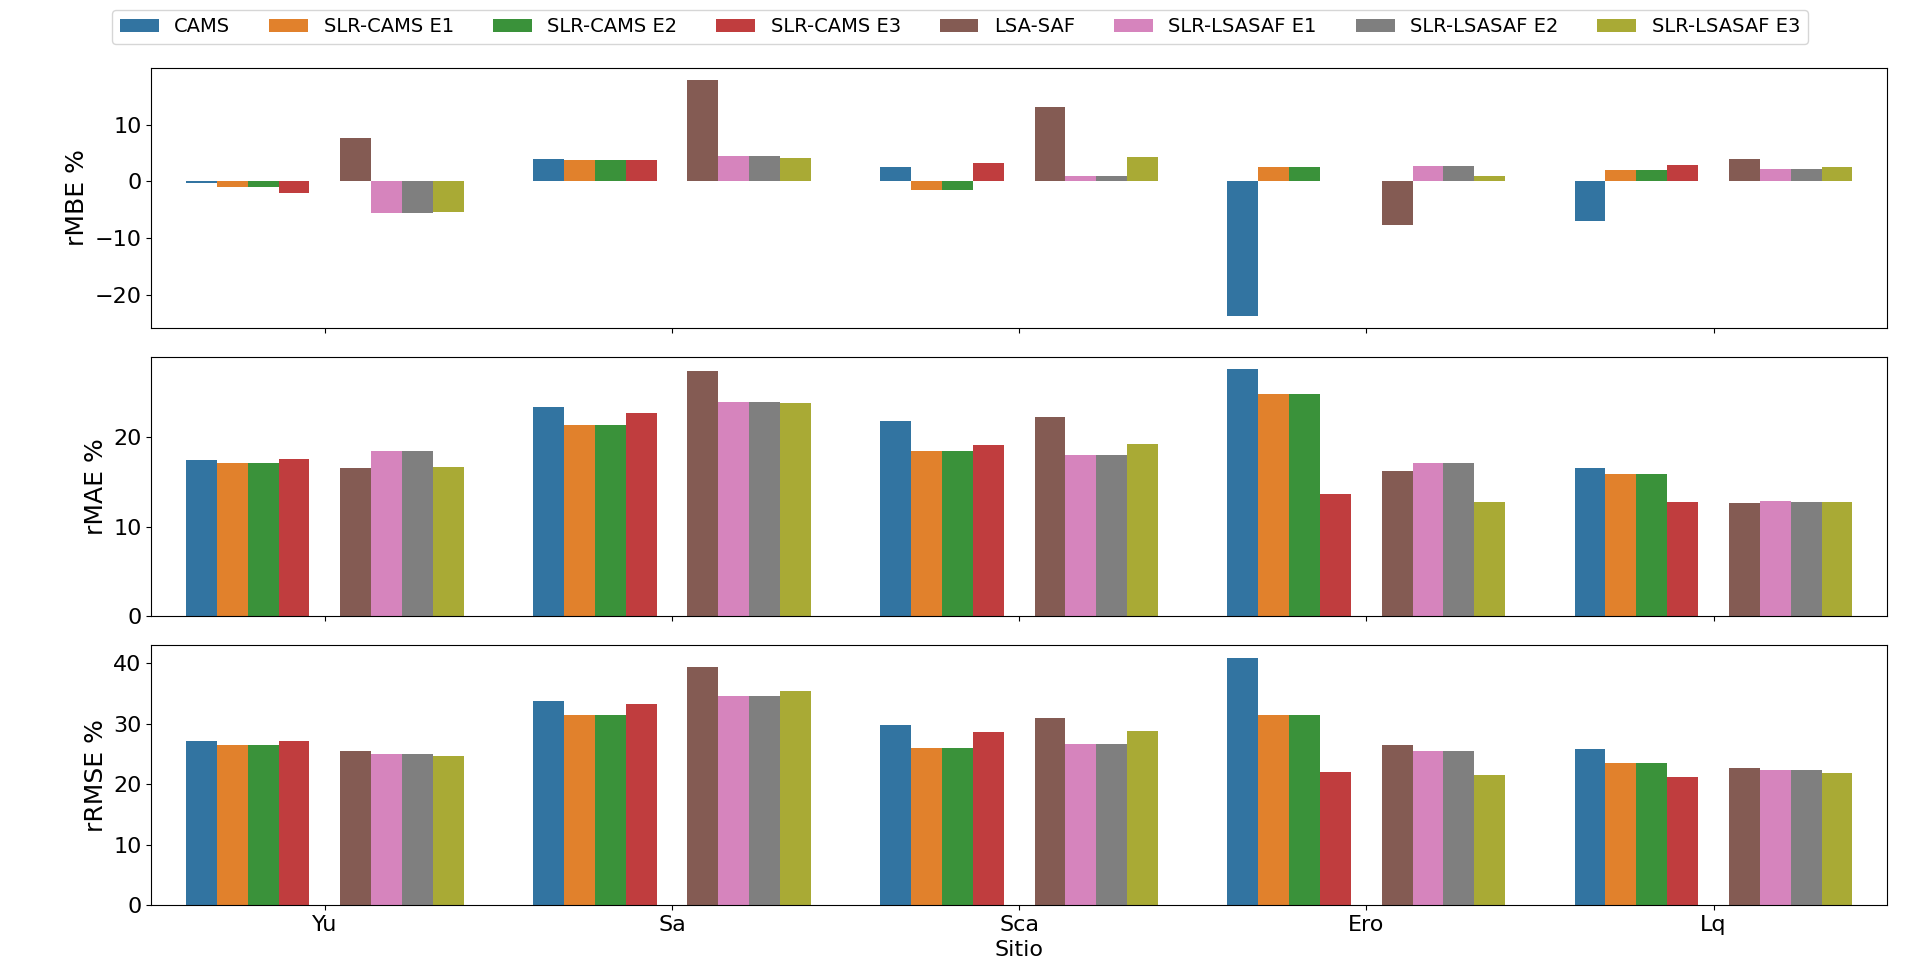
\includegraphics[width=\textwidth]{errors_estacionalidad.png}
    \caption{Métricas de desempeño relativas (\textit{rMBE}, \textit{rMAE} y \textit{rRMSE}, en \%) obtenidas en los cinco sitios de prueba (Yu, Sa, Sca, Ero y Lq). 
    Se comparan las estimaciones satelitales originales (CAMS y LSA-SAF) con sus adaptaciones al sitio mediante los enfoques E1, E2 y E3. 
    En cada subplot se agrupan las barras por sitio, mostrando primero los modelos basados en CAMS y luego, separados visualmente, los modelos basados en LSA-SAF.}
    \label{fig:metricas_estacionalidad}
\end{figure}


La Tabla \ref{tab:metricas_4_1} y la Figura \ref{fig:metricas_estacionalidad} muestran las métricas de desempeño obtenidas tras evaluar los tres enfoques sobre la desestacionalización de la serie. Se comparan las estimaciones satelitales originales (CAMS y LSA-SAF) con sus adaptaciones al sitio mediante los enfoques E1, E2 y E3. Cada subplot corresponde a una métrica distinta, y dentro de cada sitio se presentan primero los modelos basados en CAMS y luego, separados visualmente, los basados en LSA-SAF.

En general, los enfoques 1 y 2 muestran métricas bastante similares, lo que sugiere que ambos logran capturar de manera equivalente las correcciones sistemáticas del modelo; sin embargo, podrían no ajustarse perfectamente a sitios con variaciones estacionales más complejas o patrones de error no lineales.

El Enfoque 3, que desestacionaliza tanto la variable regresora como la objetivo utilizando la GHI de cielo claro, tiende a mejorar de manera consistente la estimación original y resulta especialmente útil en sitios con alta variabilidad estacional, como Ero y Lq. No obstante, en sitios con nubosidad persistente o cobertura irregular, la desestacionalización puede ser menos efectiva, ya que los patrones estacionales quedan parcialmente enmascarados por la frecuente presencia de nubes, lo que dificulta capturar con precisión las fluctuaciones de la GHI. A pesar de esta limitación, el Enfoque 3 mantiene la capacidad de corregir errores dependientes del ciclo solar y, incluso en los casos menos favorables, logra mejorar la estimación original respecto a los modelos sin adaptación.









